\documentclass[11pt]{article}
\usepackage[a4paper,margin=25mm]{geometry}
\usepackage[T1]{fontenc}
\usepackage[utf8]{inputenc}
\usepackage{lmodern}
\usepackage{graphicx}
\usepackage{booktabs}
\usepackage{amsmath}
\usepackage{xspace}
\usepackage{hyperref}
\renewcommand{\topfraction}{0.9}
\renewcommand{\bottomfraction}{0.9}
\renewcommand{\textfraction}{0.1}
\graphicspath{{figs/}}
\newcommand{\code}[1]{\texttt{#1}}
\newcommand{\us}{\textmu s\xspace}
\newcommand{\Na}{\ensuremath{{}^{22}\mathrm{Na}}\xspace}

\title{BGO scan: the Antarctica runs}
\author{J.\,J.~Gómez-Cadenas}
\date{15 October 2026}

\begin{document}
\maketitle

\begin{abstract}
This note describes the analysis of the \emph{Antarctica runs} (196~K,
$-77\,^\circ$C) taken with our test BGO crystal ($48 \times 48 \times 20$ mm$^3$),  read out by 
64 Hamamatsu S14160-6050HS SiPMs. The two runs were taken at 41 and 40.5~V of bias, 6.5 and 6.0~V of overvoltage.
A \Na\ source was located about 3 cm from the crystal's center. The BGO was fully wrapped in Teflon, and
cooled to the nominal temperature, with three different thermometers providing actual readings in different parts of the setup. The trigger required a majority of two channels above the noise (20 counts).

The data show that 12 channels were dead, a major hurdle that requires repeating the measurement. The data are also noisy. The noise of each channel grows towards low frequencies below 1 MHz and is white above it. This low-frequency noise is identical in the biased and the unbiased channels, indicating that it comes from front-end electronics. At 41 V I can measure the SPE in a respectable fraction of channels (45 out of 52 live channels) using dark pulses. The measurement shows 4 channels with very high gain, and relative uniformity for the rest. The bias of the trigger on the events depends on the operating voltage of the SiPMs. The photoelectric peak is visible in the two runs examined here, but not in a third run at 39 V, where the single-photoelectron pulse falls below the threshold and the trigger loses the 511 keV events.

The energy resolution at 511 keV is dominated by the dependence of the light collection on the position of the interaction, due to the inhomogeneity introduced by the dead channels (a fifth of the active readout is dead, creating an effective hole in the crystal). Correcting for this effect yields 22\% FWHM; the electronic noise contributes about 15\%, which leaves about 16\% once subtracted (both effects can be mitigated but not fully eliminated). The scintillation decay time at 196 K is 2.74 $\pm$ 0.01~\us.
\end{abstract}

\section{Introduction}

\subsection{The detector}
\label{sec:channels}

\begin{figure}[tbhp!]
\centering
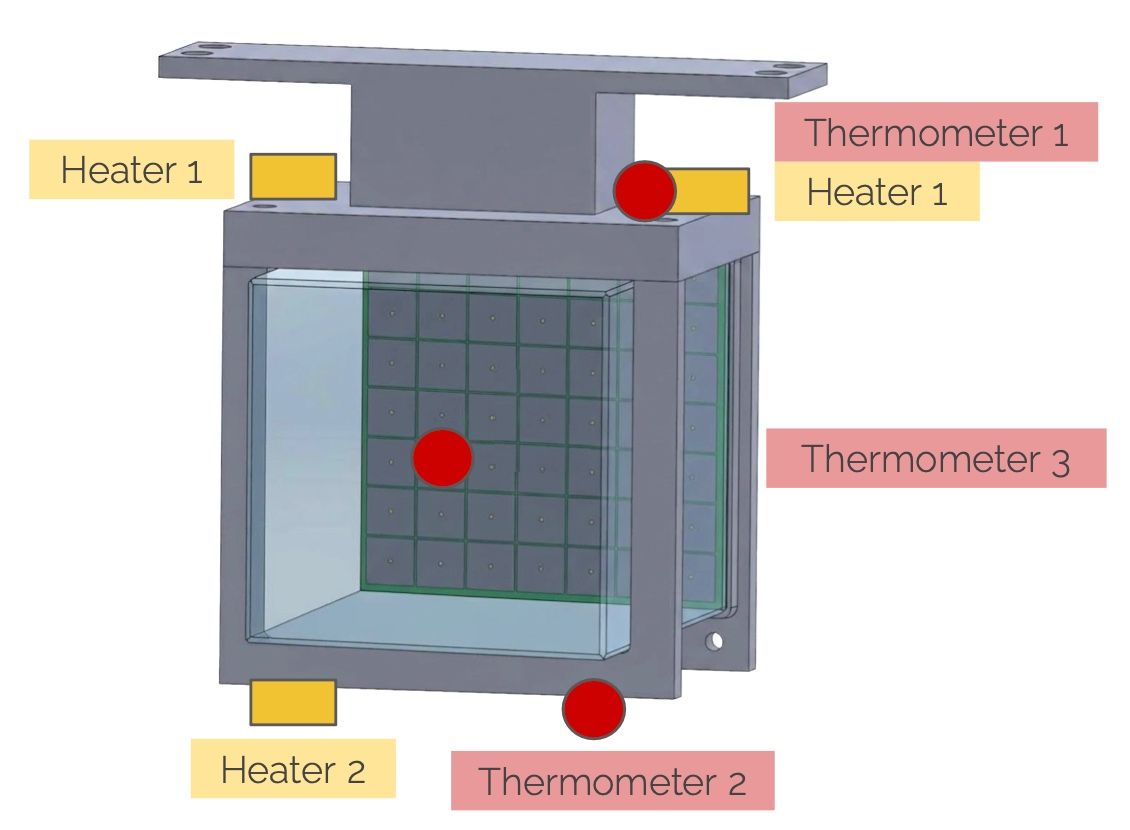
\includegraphics[width=0.6\linewidth]{figs/thermometers.jpg}
\caption{A drawing showing the setup. }
\label{fig:det}
\end{figure}

The detector (Fig. \ref{fig:det}) is a BGO crystal of $48 \times 48$~mm$^2$ and 20~mm thickness,
wrapped in Teflon on all faces but one. That face is read out by 64
Hamamatsu S14160-6050HS SiPMs of $6 \times 6$~mm$^2$, arranged in an $8
\times 8$ matrix. 

The crystal is placed inside an aluminium frame and wrapped in Teflon except in the readout face. The system is in thermal contact with a LN$_2$ reservoir. The target temperature are achieved using heaters which warm the frame, one located at the top plate and one located at
the bottom. Thermometer read the temperature on the top plate, thermometer 2 the temperature at the bottom
of the frame, and thermometer 3 at the centre of the back face, between the
Teflon and the SiPM array.

A source of \Na, placed about 3 cm from the crystal center, emits a gamma pair  of
511~keV and a single gamma of 1275~keV.

\begin{figure}[tbhp!]
\centering
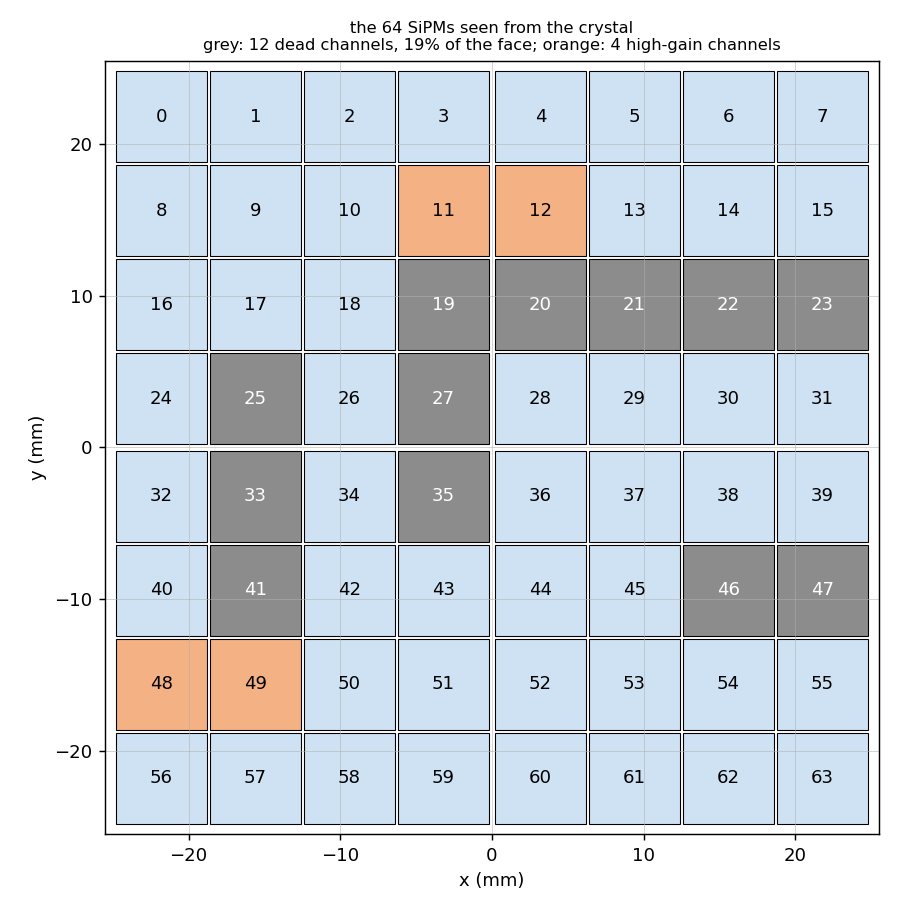
\includegraphics[width=0.6\linewidth]{chanmap.png}
\caption{The 64 SiPMs seen from the crystal, labelled with their
digitizer channel. Grey: the twelve dead channels. Orange: the four
high-gain channels (\code{chanmap.py}).}
\label{fig:chanmap}
\end{figure}

Figure~ \ref{fig:chanmap} shows a map of the SiPMs. Twelve channels are dead, creating an effective hole in the middle of the crystal. Four channels (48, 49, 11 and 12) have an abnormal high gain. 
The channels are not all alike, and the single event of


\begin{figure}[tbhp!]
\centering
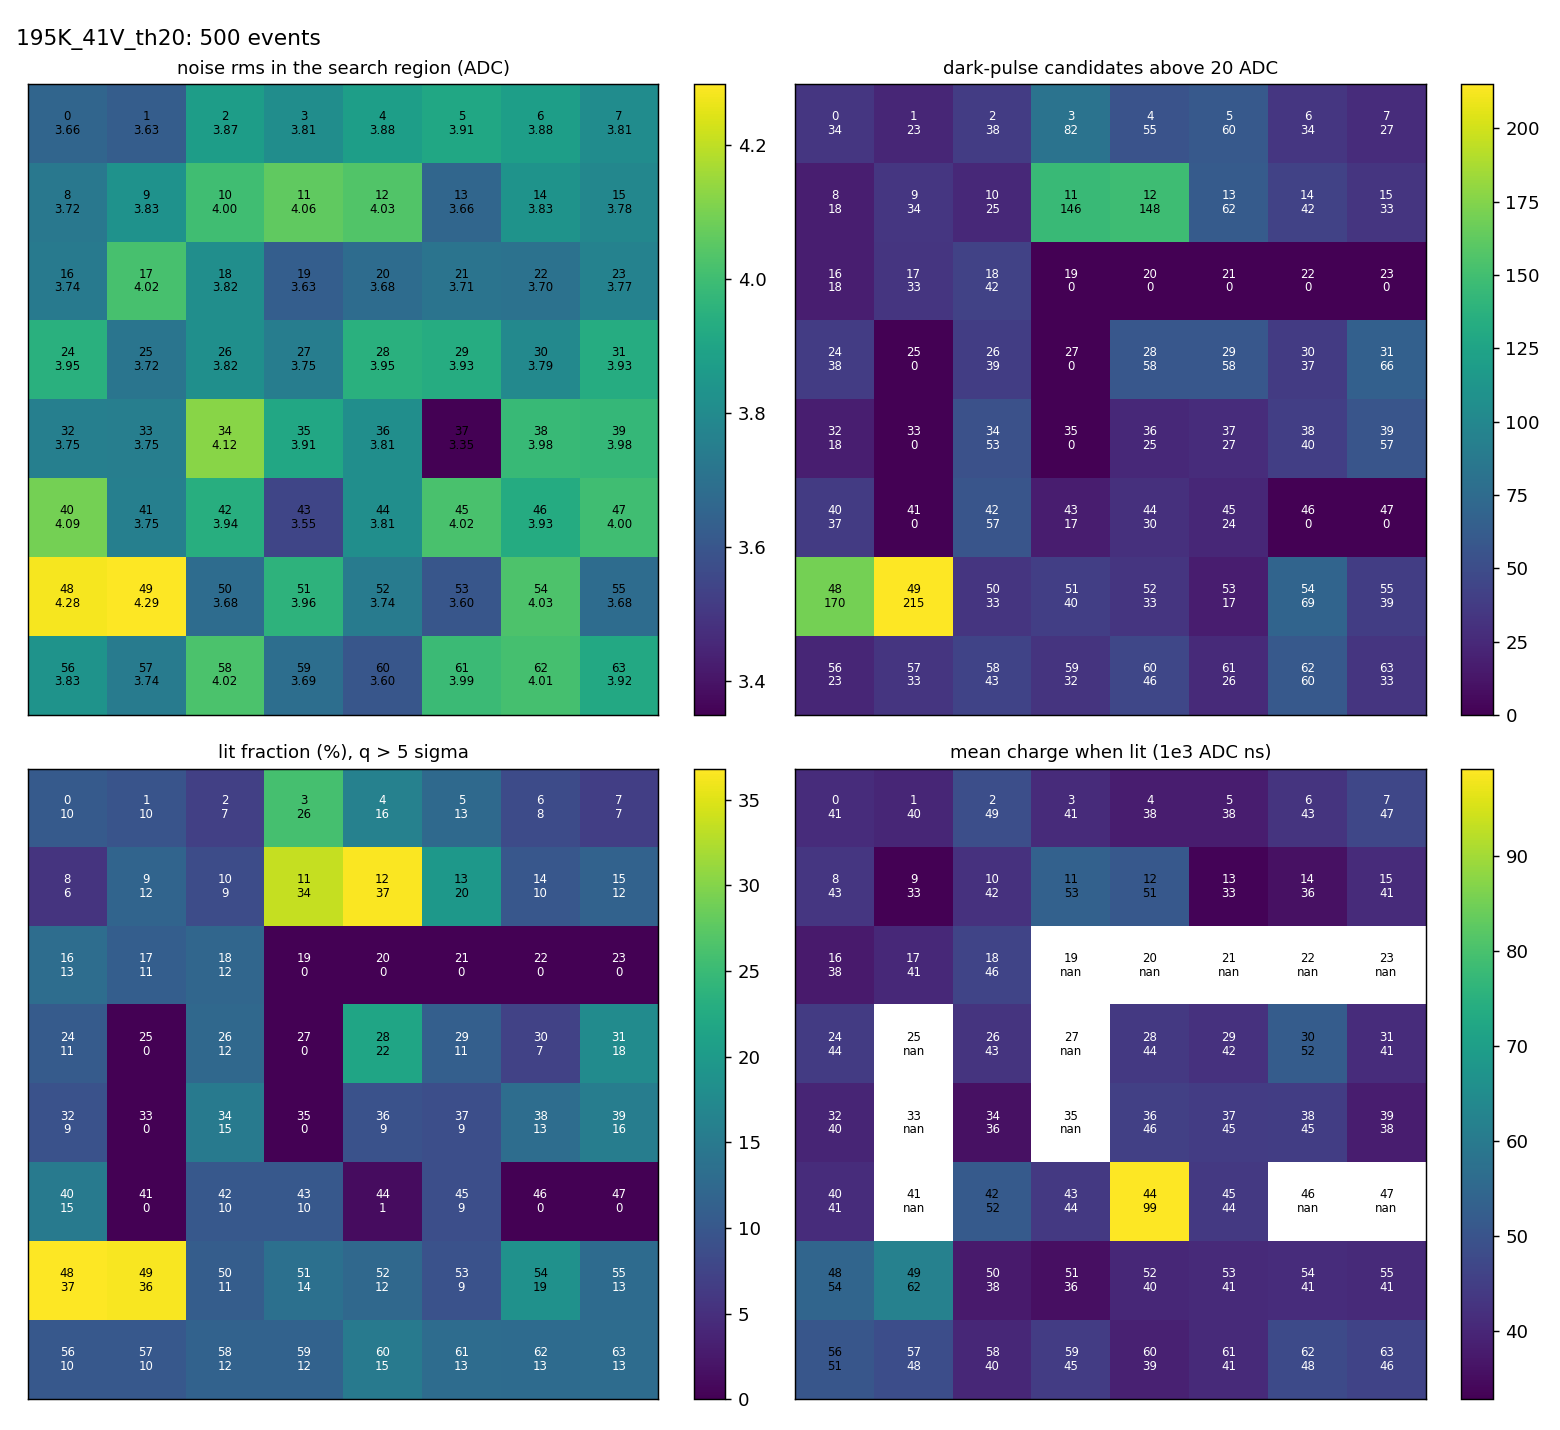
\includegraphics[width=\linewidth]{figs/chanstat_195K.png}
\caption{Maps of channel response.}
\label{fig:chanstat}
\end{figure}


Figure~\ref{fig:chanstat} shows four maps of the channels accumulated over
500 events of the run at 195~K and 41~V. On the top left the noise of each channel in the
last 10~\us of its records ---no scintillation light--- is shown; top right, shows the
number of dark pulses above 20 counts; bottom left displays the fraction of events
in which the channel carries a significant charge in the signal
window ($S/N >5$); the bottom right panel shows and the mean charge for events where $S/N >5$.
The noise is uniform, 3.4 to 4.3 counts rms per channel.
Twelve channels are dead: 19 to 23, 25, 27, 33, 35, 41, 46 and 47
(see Figure ~\ref{fig:chanmap}). 
Four channels, 11, 12, 48 and 49, have abnormal high gain. 
Channel 44 is particularly troublesome. It has normal noise and dark pulses but a charge noise too high and its
baseline wanders slowly.

\subsection{The scan}
\label{sec:data}

Twelve runs of 5000 events each were taken, at temperatures from
128 to 197~K (Table~\ref{tab:runs}). Along the temperature scan the bias
was raised with the temperature, from 37 to 41~V in steps of 1~V, to keep
the overvoltage of the SiPMs nominally constant. Two bias scans were added
at the highest temperature: at about 185~K the bias was lowered from 40~V to 38.5~V in
steps of 0.5~V, and at about 196~K from 41~V to 39~V, each step a run of
5000 events. The runs are named after the crystal temperature, the bias and
the trigger threshold: \code{185K\_39d5V\_th19} is 185~K, 39.5~V, 19 ADC
counts.

PLOT HERE. 

\begin{table}[tbhp!]
\centering
\label{tab:runs}
\begin{tabular}{l l r r r r r r}
\toprule
run & start & T1 & T2 & T3 & bias (V) & threshold & trigger rate \\
\midrule
253K\_41V\_th22   & 11:17 & 247.0 & 253.4 & 253.2 & 41.0 & 22 & \\
128K\_37V\_th19   & 14:47 & 131.0 & 131.8 & 128.6 & 37.0 & 19 & 1.9 kHz \\
153K\_38V\_th19   & 14:54 & 161.6 & 157.5 & 153.1 & 38.0 & 19 & 20 kHz \\
164K\_39V\_th19   & 15:00 & 170.7 & 172.9 & 164.8 & 39.0 & 19 & 66 kHz \\
184K\_40V\_th19   & 15:13 & 180.7 & 190.1 & 184.8 & 40.0 & 19 & 132 kHz \\
185K\_39d5V\_th19 & 15:15 & 181.0 & 190.1 & 185.8 & 39.5 & 19 & 80 kHz \\
186K\_39V\_th19   & 15:16 & 181.2 & 190.2 & 186.6 & 39.0 & 19 & 43 kHz \\
187K\_38d5V\_th19 & 15:17 & 181.5 & 190.2 & 187.4 & 38.5 & 19 & 19 kHz \\
195K\_41V\_th20   & 15:28 & 183.7 & 205.0 & 195.8 & 41.0 & 20 & 225 kHz \\
196K\_40d5V\_th20 & 15:29 & 183.8 & 203.9 & 196.2 & 40.5 & 20 & 148 kHz \\
196K\_40V\_th20   & 15:30 & 183.9 & 203.1 & 196.6 & 40.0 & 20 & 97 kHz \\
196K\_39d5V\_th20 & 15:33 & 184.0 & 202.5 & 196.9 & 39.5 & 20 & 29 kHz \\
197K\_39V\_th20   & 15:35 & 184.1 & 201.9 & 197.3 & 39.0 & 20 & 2.7 kHz \\
\bottomrule
\end{tabular}
\caption{The runs, in order of acquisition, with the three thermometer
readings in kelvin, the SiPM bias and the
trigger threshold. The last column is the true trigger rate.}
\end{table}

The temperatures were not stable and 
the frame had a vertical gradient at high temperatures. The SiPM board is mounted on the frame, and therefore
 the SiPMs were probably warmer than the crystal, somewhere between T3 and T2. This has an effect on the
 overvoltage, which depends on the SiPM temperature, as I will discuss below. 
\subsection{The two runs}
\label{sec:sipm}

The S14160-6050HS is a 6~mm SiPM with 50~\textmu m pixels and a low breakdown
voltage. The datasheet gives, at 25~\textdegree C: breakdown voltage
$V_{\rm bd} = 38$~V, recommended operation at $V_{\rm bd} + 2.7$~V, a
temperature coefficient of the breakdown of 34~mV/K, gain $2.5 \times 10^6$
at 2.7~V overvoltage and growing linearly with it (about $0.9 \times 10^6$
per volt), photon detection efficiency 50\% at 2.7~V and nearly saturated
above 3~V, crosstalk 7\%. Each SiPM is read through a shaper into the
50~$\Omega$ input of the digitizer; the details of the shaper are not
known to us yet. Its effect is visible in the data: a single
photoelectron is a pulse 24~ns wide at half maximum (Section~\ref{sec:spe}),
much faster than the 2~nF of a bare 6~mm SiPM into 50~$\Omega$ would give.

The bias was set from the datasheet values and a best guess for each
temperature; the breakdown voltage was never measured. We can therefore
only estimate the overvoltage. Extrapolating the datasheet coefficient from
298~K, $V_{\rm bd}(T) = 38~\mathrm{V} + 0.034~\mathrm{V/K}\,(T - 298~\mathrm{K})$,
and taking the SiPM temperature equal to T3, the overvoltage of the five
runs along the temperature scan is 4.8, 4.9, 5.5, 5.8 and 6.5~V at 129,
153, 165, 185 and 196~K: the bias rose by 60~mV/K while the breakdown rose
by 34~mV/K, so the overvoltage was not constant but grew by 35\% along the
scan. The lowest points of the bias scans, 38.5~V at 187~K and 39~V at
197~K, are at 4.3 and 4.4~V. No run is near breakdown.

If the SiPMs were warmer than the crystal, their breakdown was higher and
their overvoltage lower than these numbers. Taking the SiPM temperature
halfway between T3 and T2 lowers the overvoltages by 0.1~V at 128~K and by
0.15~V at the warm end; taking it equal to T2 lowers them by 0.1 to 0.3~V.
This is a small uncertainty next to the 1.7~V rise along the scan. What
the uncertainty of the overvoltage means for the analysis is that the
light yield measured in ADC counts contains a gain factor that changes
from run to run, mostly through the SiPM gain, since the photon detection
efficiency is saturated above 3~V. The factor has to be measured, and the
bias scans and the single-photoelectron response are the two handles
(Section~\ref{sec:spe}).

The two runs of this note are \code{195K\_41V\_th20} and
\code{196K\_40d5V\_th20}, the first two of the bias scan at 196~K. Both
hold the 511~keV line intact: the trigger threshold of 20 counts sits
below the single-photoelectron pulse only at these two biases, 20.7
counts at 41~V and about 19 at 40.5~V, and at lower bias the 511~keV
events stop triggering (\code{ANALYSIS.md}, 2026-10-15). The 41~V run
carries the gain table and the clearest 1275~keV line; the 40.5~V run
has a fifth of the pile-up and is the control.

\begin{table}[h]
\centering
\begin{tabular}{l c c c c c c c}
\toprule
Run & Bias & T1 & T2 & T3 & Overvoltage & Trigger rate & Events \\
 & (V) & (K) & (K) & (K) & at T3 (V) & (kHz) & \\
\midrule
195K\_41V\_th20   & 41.0 & 183.7 & 205.0 & 195.8 & 6.5 & 225 & 5000 \\
196K\_40d5V\_th20 & 40.5 & 183.8 & 203.9 & 196.2 & 6.0 & 148 & 5000 \\
\bottomrule
\end{tabular}
\caption{The two runs of this note.}
\end{table}

\subsection{The acquisition}
\label{sec:daq}

The digitizer is a CAEN DT2745 with the Scope firmware, 64 channels at 125
MHz and 16 bits, read by WebDump. Each event is a record of 3000 samples
(24~\us) per channel, 200 of them (1.6~\us) before the trigger. The
trigger is internal: a channel fires when it rises above its baseline by
the threshold, 19 counts in the cold runs and 20 in the warm ones, and the
event is accepted when at least two channels fire in coincidence (majority
2). The records hold the raw ADC counts; the per-channel baselines measured
by WebDump at the start of the run are stored with them.

The first thing the data show is that the readout, not the trigger, set
the rate at which events were recorded. Every run holds 5000 events in
40.7~s, that is 123~Hz, whatever the temperature, the bias or the
threshold, and the events come in bursts of three, 1.3~ms apart, separated
by gaps of 22.8~ms. That is a readout saturated at its throughput, about
47~MB/s: the board fills a small buffer, transfers it, and is blind in
between. The recorded rate carries no physics.

The trigger rate is nevertheless known, because the board numbers every
trigger in a 24-bit counter and the number is stored with each recorded
event. The difference between the counters of the last and the first event
of a run, modulo $2^{24}$, divided by the duration, is the rate at which the
trigger fired (Table~\ref{tab:runs} and Figure~\ref{fig:rates}). It goes
from 1.9~kHz at 128~K and 37~V to 225~kHz at 196~K and 41~V, and it rises
steeply with the bias at fixed temperature: by a factor 7 from 38.5 to
40~V at 185~K, by a factor 80 from 39 to 41~V at 196~K. No source gives
hundreds of kHz in a crystal this size. The trigger was firing on the dark
pulses of the SiPMs: a dark pulse of one or two photoelectrons crosses the
threshold in one channel, and the majority logic turns the single-channel
rate into a coincidence rate that grows with its square.

\begin{figure}[tbp]
\centering
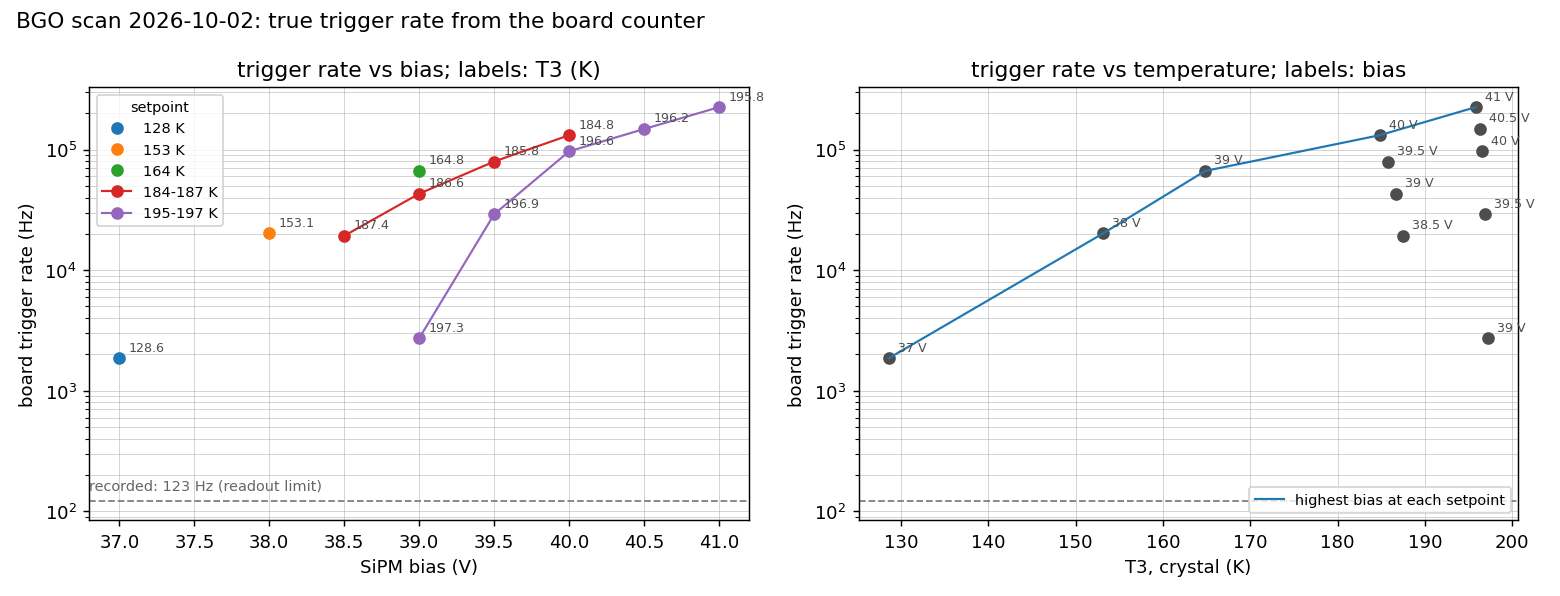
\includegraphics[width=\linewidth]{figs/scan_rates.png}
\caption{The true trigger rate of the board, from the trigger counter.
Left: against the bias, one colour per temperature setpoint, the two bias
scans joined by lines, each point labelled with its T3; the dashed line is
the recorded rate, the same in all runs. Right: against T3, each point
labelled with its bias; the line joins the five runs of the temperature
scan.}
\label{fig:rates}
\end{figure}

That it is the overvoltage and not the temperature that drives the rate
is seen at fixed bias. Three runs were taken at 39~V: the rate is 66~kHz at
165~K, 43~kHz at 187~K and 2.7~kHz at 197~K. The dark-count rate of a SiPM
grows with temperature, so at fixed overvoltage the rate would rise along
this sequence; it falls, because at fixed bias the overvoltage drops as
the breakdown voltage rises with the temperature, the gain drops with it,
and the single-photoelectron pulse falls below the threshold. The steepness
at 196~K, a factor 10 between 39 and 39.5~V, is the signature of the
threshold sitting close to the amplitude of one or two photoelectrons.

Two consequences follow. The recorded events are a random sample of the
triggers, from 7\% of them at 128~K to 0.05\% at 196~K and 41~V, so the
fraction of recorded events that contain a scintillation pulse is of the
order of the ratio of the real event rate to the trigger rate: most of them
at the cold end, and a few percent at the warm end at nominal bias. And
the trigger fires late on a real event, because a 511~keV pulse spreads
its photoelectrons over microseconds and few of them overlap in any
channel at any instant: a channel sees 7 to 13 counts at the peak against
a threshold of 19, and it crosses the threshold only when noise helps,
at a random time along the pulse. The start of the pulse is then often
before the record, or inside the 1.6~\us that precede the trigger.

\section{Structure of the events}
\label{sec:events}

\subsection{The 64 channels of one event}

Figure~\ref{fig:event_channels} shows the 64 channels of one event of the
run at 197~K and 39~V, the raw counts of each channel minus its WebDump
baseline. The light is in a dozen channels: the row 48 to 55, and 11 and
12, each with a pulse of 10 to 25 counts rising at the trigger and decaying
over a microsecond. The other channels show the noise of the chain, 3.9
counts rms per sample, white except for a correlation between neighbouring
samples (Section~\ref{sec:spe}), and here and there an isolated spike of
about 15 counts, which is a dark pulse of one photoelectron.

\begin{figure}[tbp]
\centering
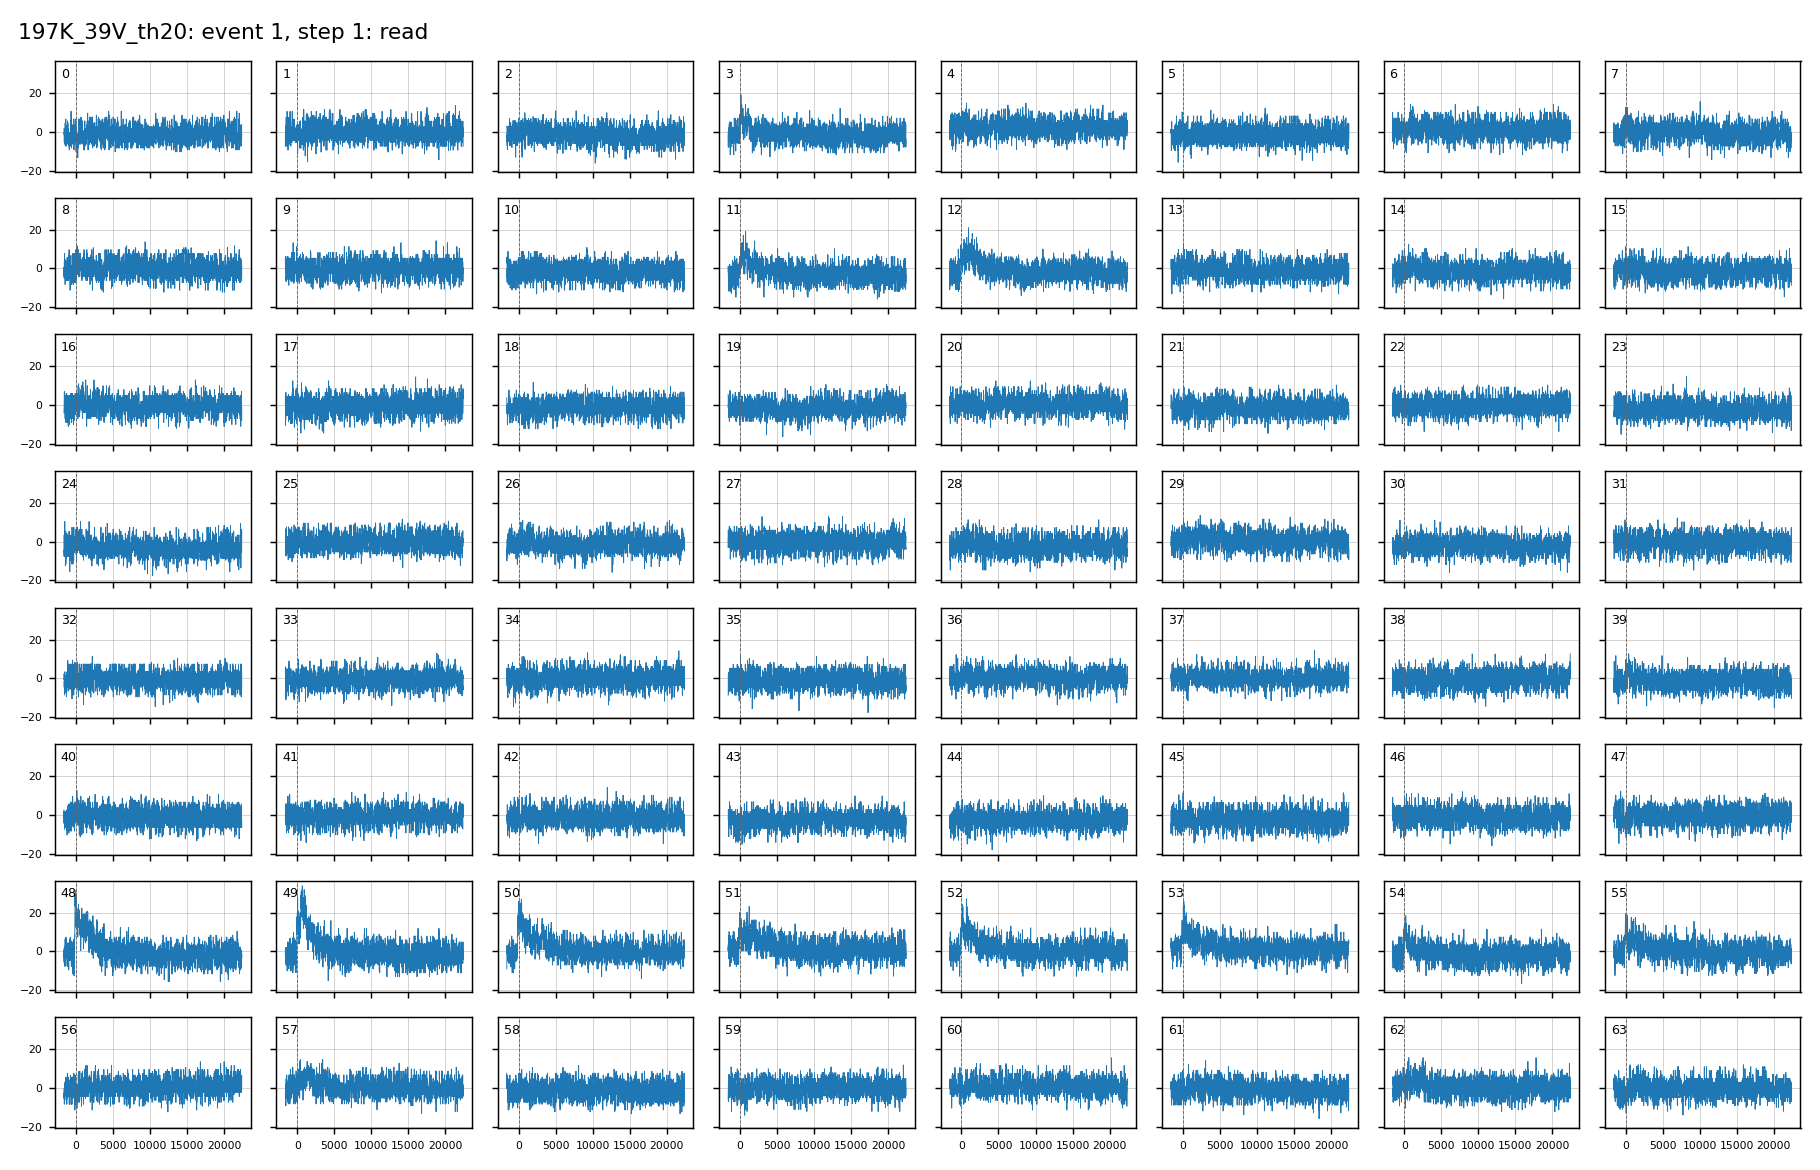
\includegraphics[width=\linewidth]{figs/sel_197K_ev1_s1.png}
\caption{Event 1 of \code{197K\_39V\_th20}: the 64 channels in channel order,
raw counts minus the WebDump baseline, against the time from the trigger
in ns. The light is in channels 48 to 55 and 11, 12.}
\label{fig:event_channels}
\end{figure}

\subsection{The sum}

Figure~\ref{fig:event_sum} shows the sum of the 64 channels of the same
event, after the correction described in the analysis note, with a moving
average over 64 samples (0.5~\us) on top. The pulse is 140 counts high
on the average, 200 on the raw sum, against 23 counts of noise per sample
in the sum; it rises at the trigger and decays in about 1~\us at this
temperature. At 128~K the decay is several microseconds long, and the
pulse is larger. The noise of the sum is what 64 channels of 3.9 counts add
up to, $3.9 \sqrt{64} = 31$, reduced by the correction: the part of the
noise that is common to all channels is small, 3\% of the variance of a
channel, and the sum is dominated by the independent white noise of the 64
channels.

\begin{figure}[tbp]
\centering
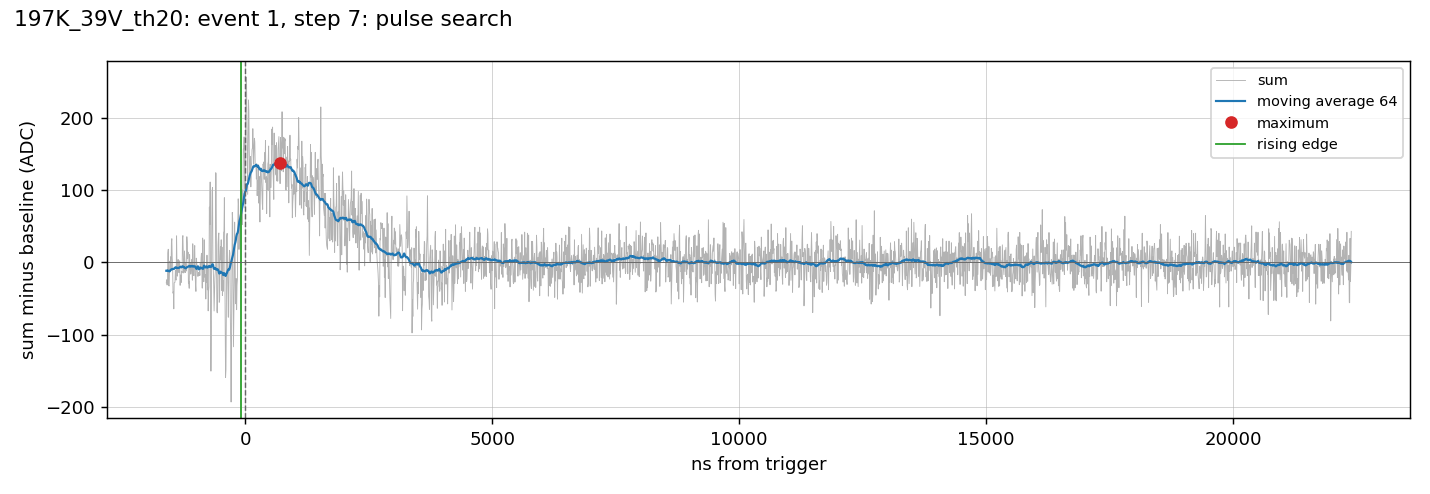
\includegraphics[width=\linewidth]{figs/sel_197K_ev1_s7.png}
\caption{The same event: the sum of the 64 channels, baseline subtracted
(grey), its moving average over 64 samples (blue), the maximum of the
average (dot) and the rising edge, where the average crosses half the
maximum (green line).}
\label{fig:event_sum}
\end{figure}

Three features of the events shape the analysis and are only named here.
The pre-trigger window is not free of signal, for the reason given in the
previous section, so the baseline of each event has to be taken from the
end of the record, 22~\us after the trigger, where the pulse is over. In
some events the pulse started before the record and only its tail was
recorded; these have to be recognised and set apart, and since small
pulses trigger later than large ones, they are lost preferentially, which
biases the spectrum. And with 24~\us of record and a real event rate of a
few kHz, a few percent of the records hold a second pulse, which has to be
found and flagged. The classification of the events, the choice of the
charge window and the definition of the charge are the first steps of the
analysis note.

\section{The structure of the noise}
\label{sec:noise}

Measured on the tail of the record, 12 to 24~\us after the trigger, where
the scintillation pulse is below 3\% of its height, on 236 clean events of
\code{195K\_41V\_th20}: REAL events without pile-up whose maximum lies more
than 4~\us before the tail (\code{cmnoise\_doc.tex},
\code{wavefit\_doc.tex}). The same measurements on \code{197K\_39V\_th20}
give the same numbers within 10\%. The expectations for white, independent
noise are drawn from simulated channels with the same geometry and rms
(\code{noisetoy\_doc.tex}).

\subsection{Noise per channel}

\paragraph{Expectation.} A channel with white noise of rms $\sigma$ per
sample has a flat power spectrum up to the Nyquist frequency, an
autocorrelation of 1 at zero lag and 0 at every other lag, and a running
mean over $N$ samples of rms $\sigma/\sqrt N$ (Figure~\ref{fig:toy1}).

\begin{figure}[tbp]
\centering
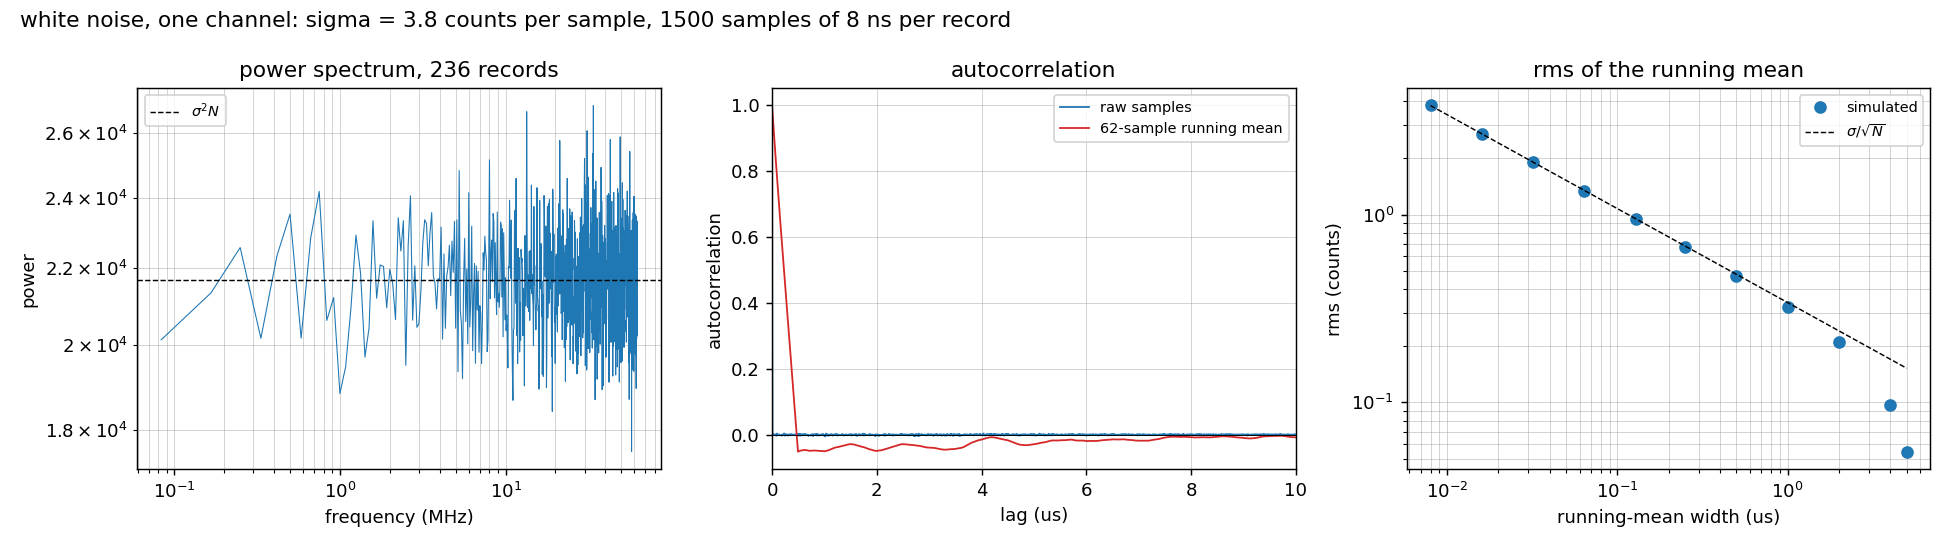
\includegraphics[width=\linewidth]{noisetoy_channel.png}
\caption{White noise, one simulated channel, $\sigma = 3.8$ counts, 1500
samples per record: power spectrum, autocorrelation of the raw samples
and of the 62-sample running mean, rms of the running mean against its
width.}
\label{fig:toy1}
\end{figure}

\paragraph{Measurement.} Per channel, over the tail: the rms per sample,
the autocorrelation at lags of a few samples, the power spectrum averaged
over events, the autocorrelation of the 62-sample running mean averaged
over events and channels, and the rms of the running mean against its
width.

\paragraph{Observation.} At the scale of the samples, as measured for
the single photoelectron:

A single photoelectron is 15 to 20 counts high on 3.9 counts of noise per
sample: a 4 to 5~sigma object if one looks at one sample. The standard
remedy is a matched filter, a weighted sum of consecutive samples with the
pulse shape as weights, which for white noise improves the signal to noise
by the square root of the sum of the squared weights, 1.5 for this pulse.
The dead channels, which hold nothing but noise, allowed us to measure the
noise rather than assume it (Figure~\ref{fig:noise}). It is correlated
between neighbouring samples, 0.43 at one lag and 0.16 at two, nothing
beyond, and its power spectrum is nearly flat up to the Nyquist frequency of
62.5~MHz, like the spectrum of the pulse itself: the pulse occupies the
same band as the noise. The matched filter then gains 1.09, and the best
linear filter for this noise, the matched filter applied after whitening,
gains 1.17; both predicted from the measured noise and verified on the dead
channels. There is no filter that makes the single photoelectron better
than a 5~sigma object at 41~V and a 4~sigma object at 39~V. This is a
property of the chain, 8~ns samples and a 24~ns pulse on 3.9 counts of
noise, and it limits what follows.

\begin{figure}[tbp]
\centering
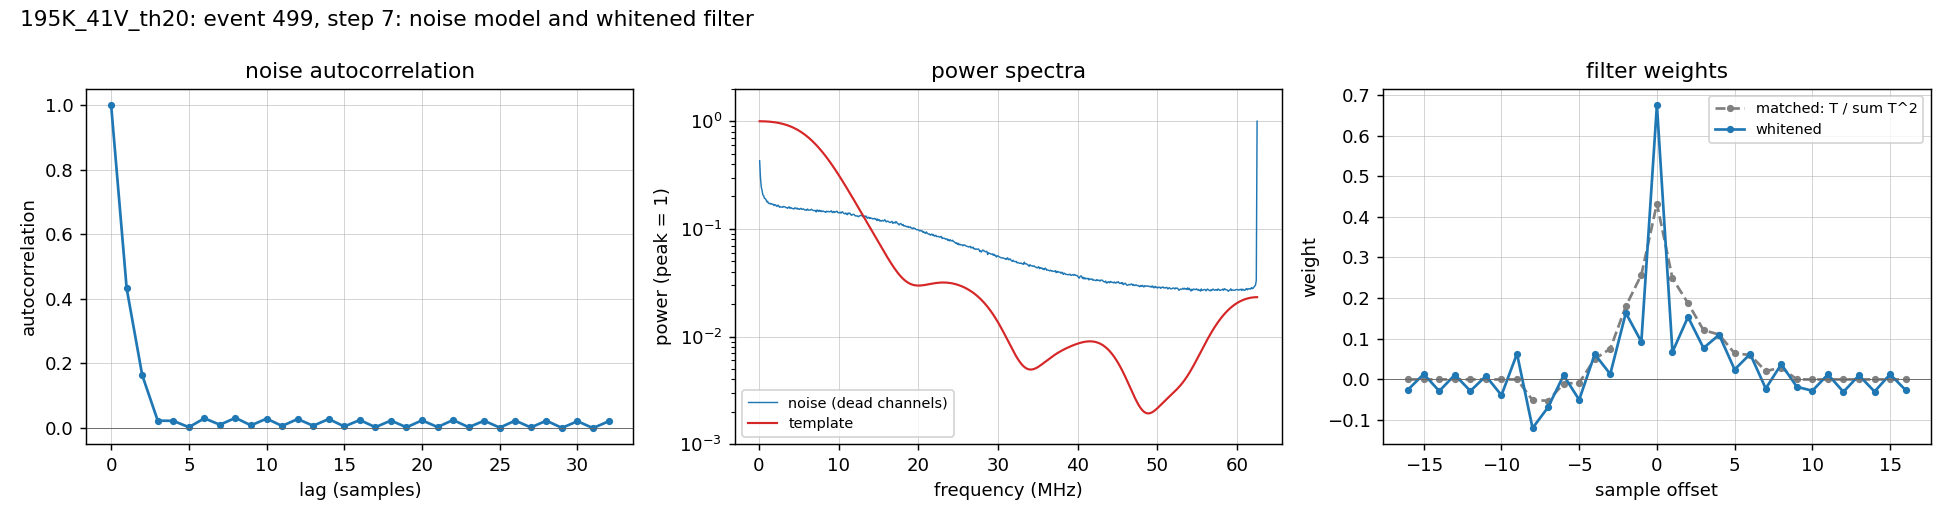
\includegraphics[width=\linewidth]{figs/tpl_195K_s7.png}
\caption{The noise of a channel, from 6000 segments of 10~\us of the
twelve dead channels. Left: autocorrelation against the lag in samples.
Centre: power spectrum, and the spectrum of the pulse template on the same
axis. Right: the weights of the matched filter and of the whitened filter
over a window of 33 samples.}
\label{fig:noise}
\end{figure}

Below 1~MHz the spectrum rises as $1/f$ (Figure~\ref{fig:spectra}). The rise is a slow
component: the rms of the running mean sits above $\sigma/\sqrt N$ from
30~ns on, by a factor 2.5 at 1~\us, and its autocorrelation reaches zero
at a lag of 1.5~\us (Figure~\ref{fig:autocorr}). The twelve dead channels
give the same spectrum, the same autocorrelation and the same
running-mean rms as the live ones (Figure~\ref{fig:traces}): both
components are in the front-end or the digitizer.


\begin{figure}[tbp]
\centering
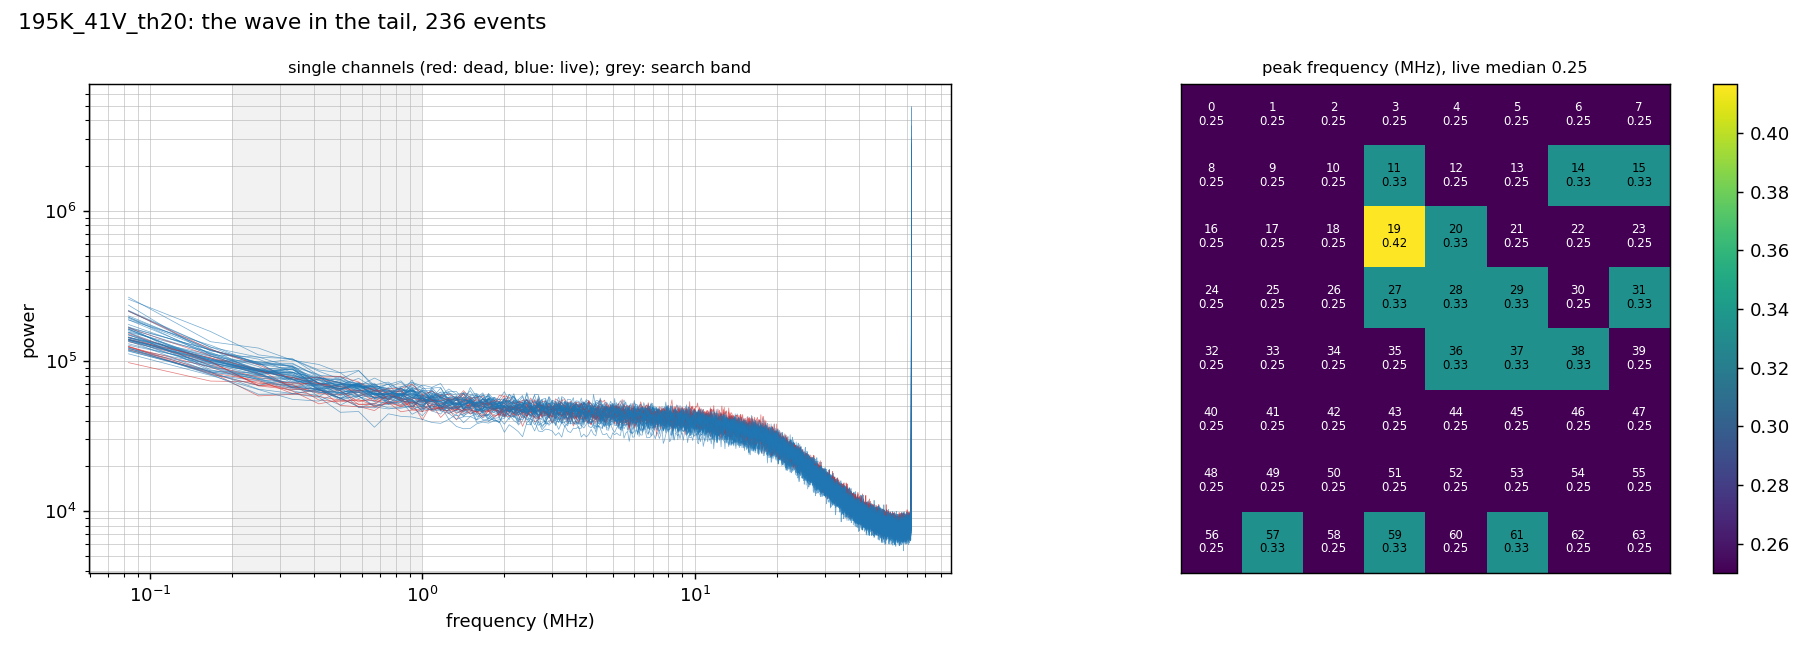
\includegraphics[width=\linewidth]{wavefit_195K_spectra.png}
\caption{The 64 single-channel power spectra over the tail, dead in red,
live in blue; the grey band is the search band of \code{wavefit.py}. Right:
the frequency of the maximum in that band per channel, the lower edge of
the band in nearly every channel.}
\label{fig:spectra}
\end{figure}

\begin{figure}[tbp]
\centering
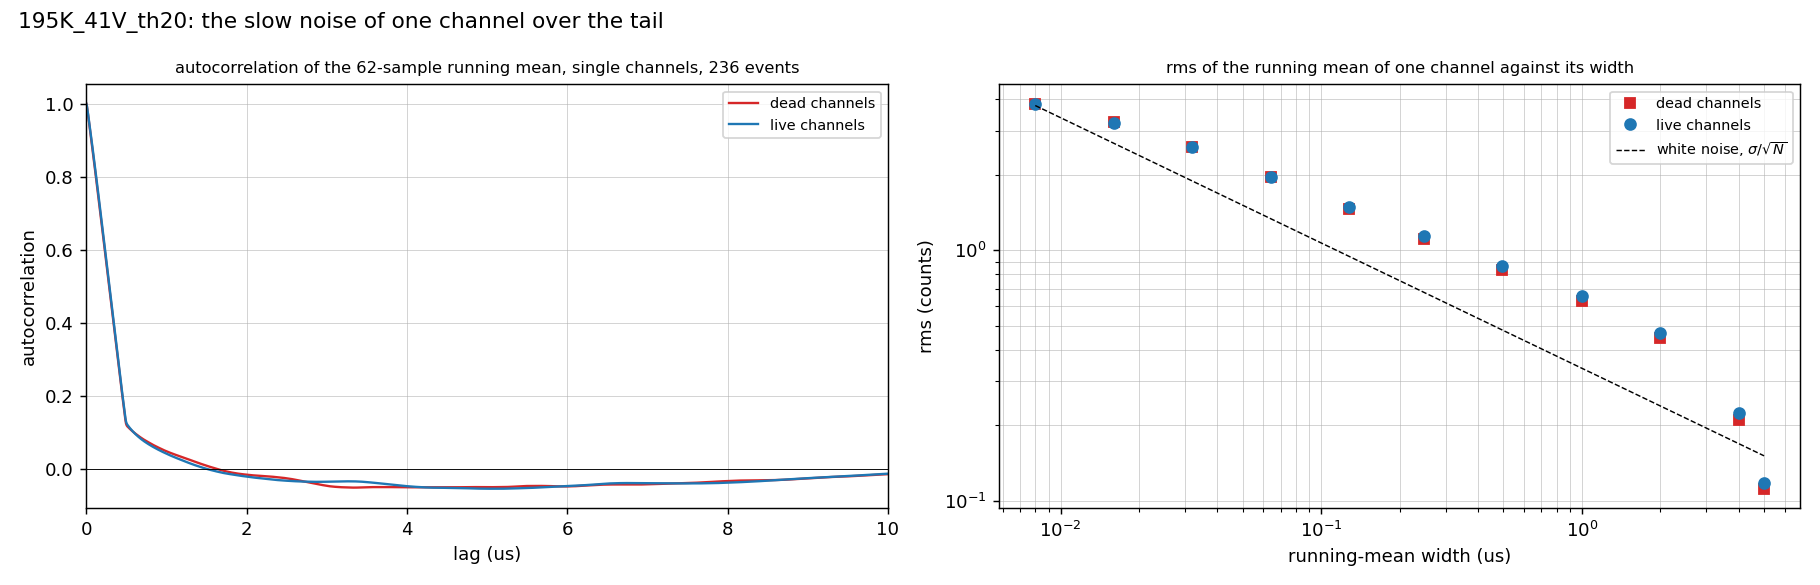
\includegraphics[width=\linewidth]{wavefit_195K_autocorr.png}
\caption{Left: autocorrelation of the 62-sample running mean of single
channels, averaged over events and over the channels of each class.
Right: rms of the running mean of one channel against its width, with
the white-noise line.}
\label{fig:autocorr}
\end{figure}

\begin{figure}[tbp]
\centering
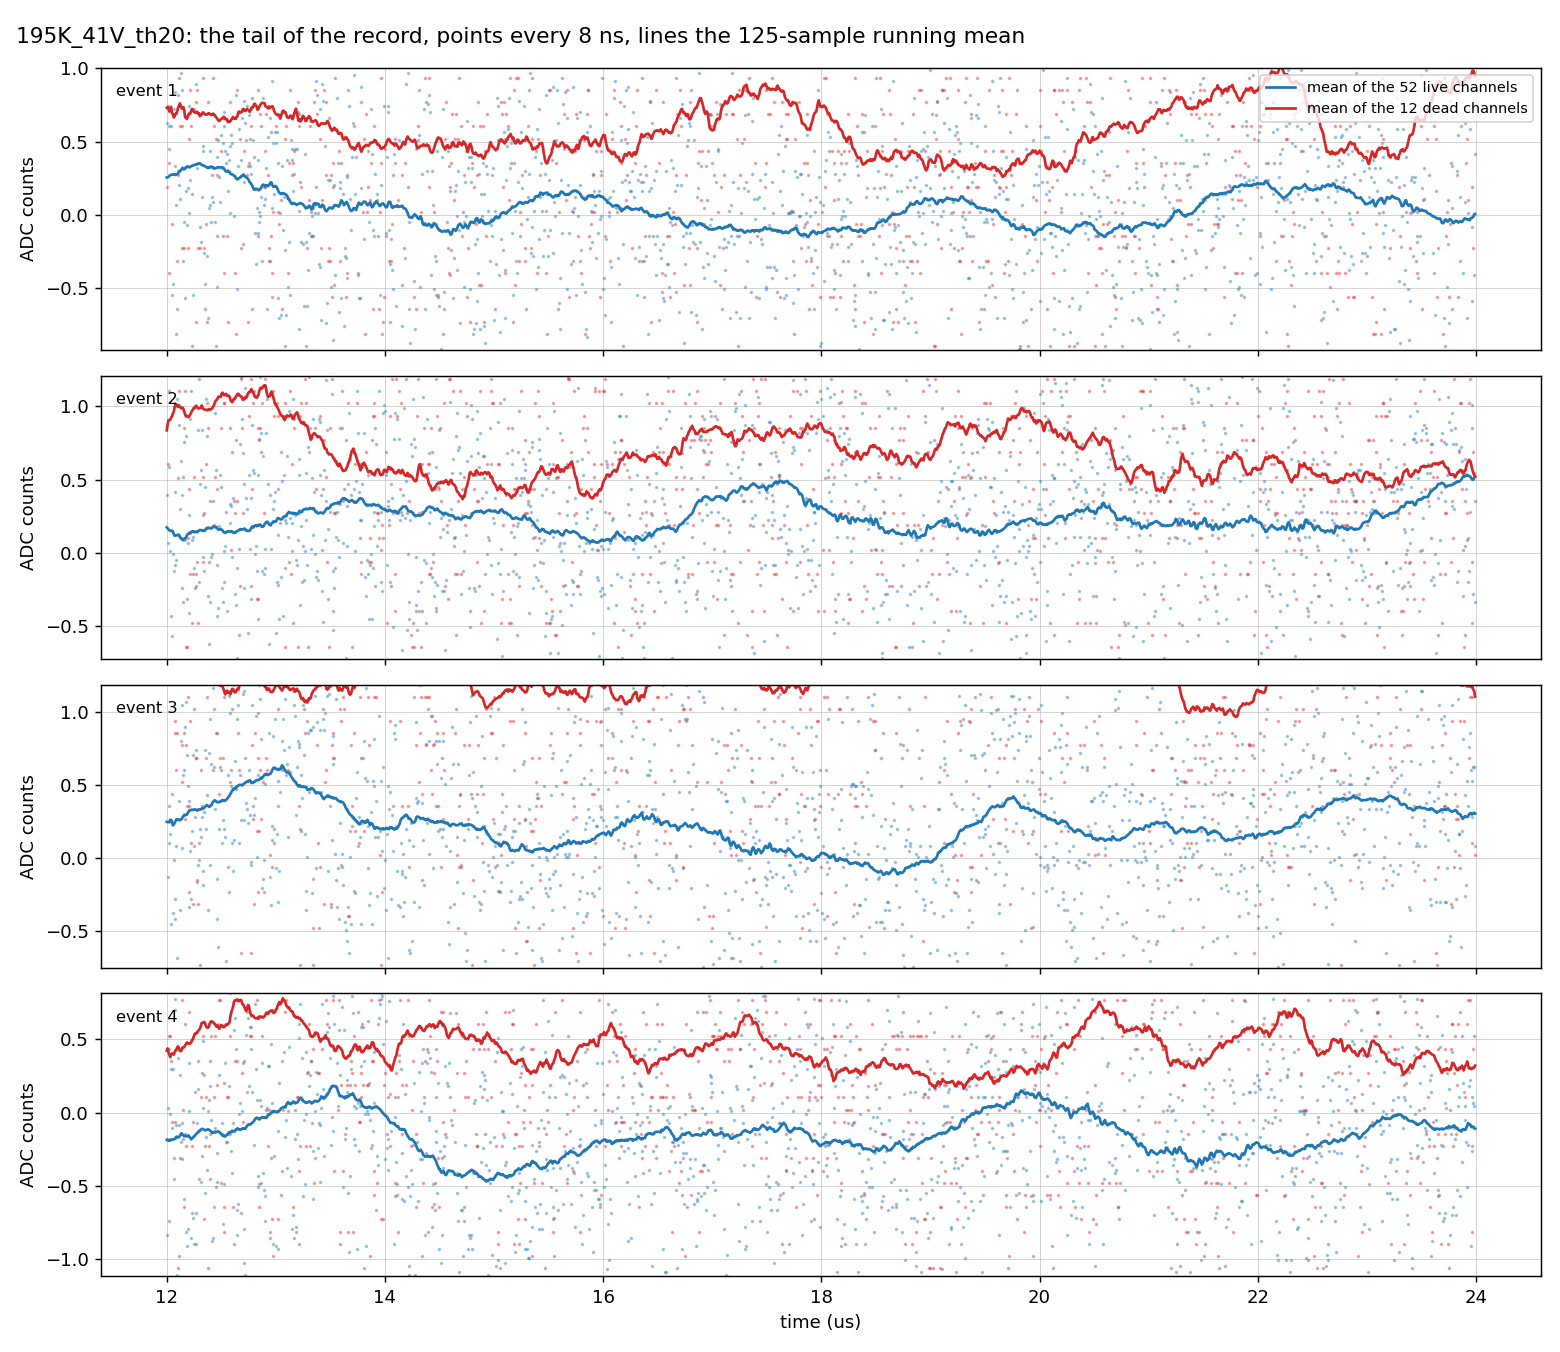
\includegraphics[width=\linewidth]{cmnoise_195K_traces.png}
\caption{Four events: the mean of the 52 live channels and of the 12 dead
channels over the tail, points every 8~ns, lines the 1~\us running mean.}
\label{fig:traces}
\end{figure}

\subsection{Correlated noise}

\paragraph{Question.} Does any part of the noise appear in several
channels at once, within a record or from record to record, and among
which channels?

\paragraph{Expectation.} For independent channels, the correlation matrix
of the running means has ones on the diagonal and zero elsewhere, within
a scatter of one over the square root of the number of samples, and the
sum of $n$ channels has an rms $\sqrt n$ times that of one
(Figure~\ref{fig:toy2}). A component common to all channels raises every
off-diagonal element to the same value and makes the sum grow towards
$n$ (Figure~\ref{fig:toy3}).

\begin{figure}[tbp]
\centering
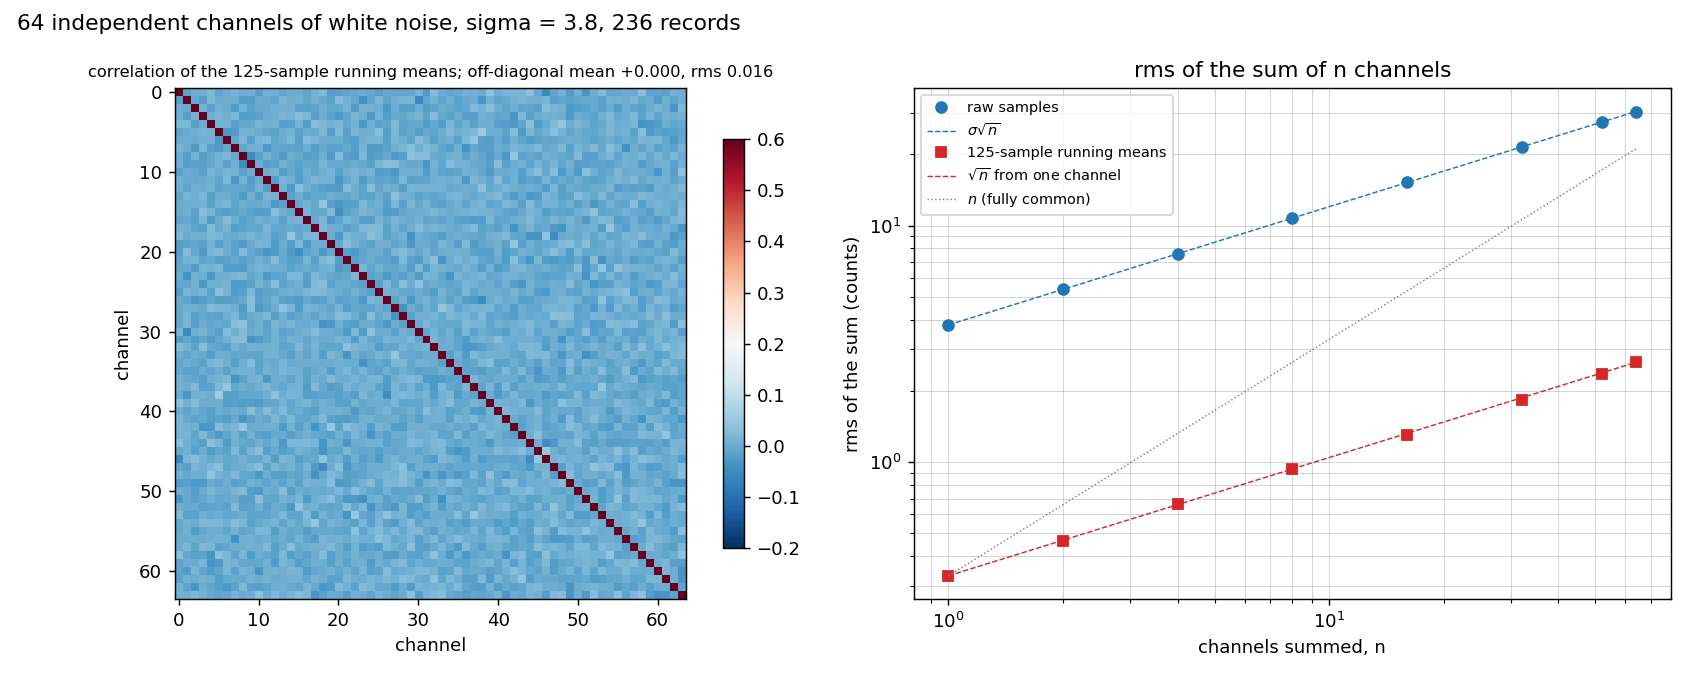
\includegraphics[width=\linewidth]{noisetoy_channels.png}
\caption{64 independent simulated channels: correlation matrix of their
125-sample running means over 236 records, and rms of the sum of $n$
channels against $n$.}
\label{fig:toy2}
\end{figure}

\begin{figure}[tbp]
\centering
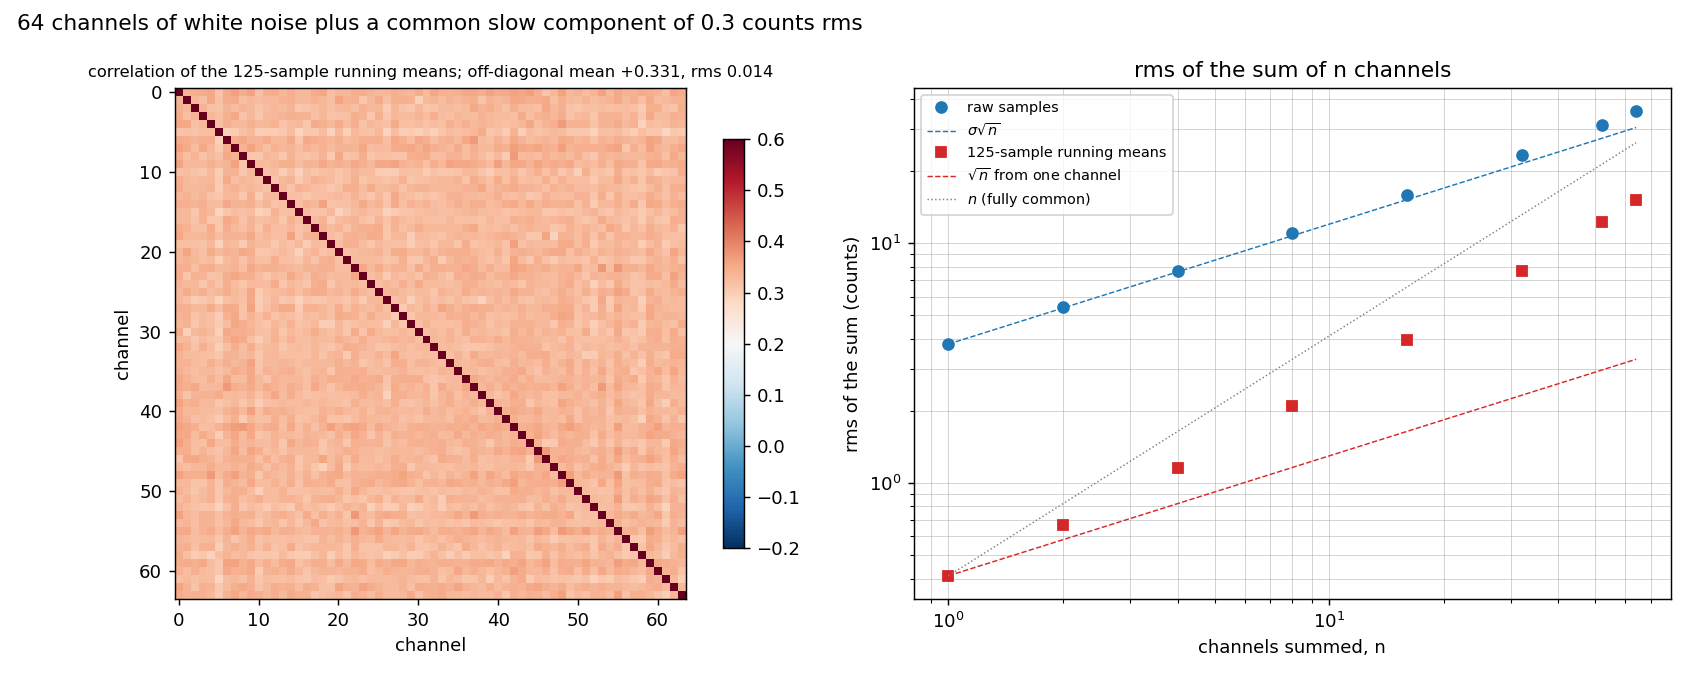
\includegraphics[width=\linewidth]{noisetoy_common.png}
\caption{The same with a slow component of 0.3 counts rms common to all
channels.}
\label{fig:toy3}
\end{figure}

\paragraph{Measurement.} The 64 by 64 correlation matrix of the 125-sample
running means over the tail, accumulated over events; the rms of the sum
of the live channels against the independent expectation; the offset of
each channel's record from the run baseline, its scatter between events
and its correlation between channels.

\paragraph{Answer.} Within a record, the channels are independent: 0.03
between live channels, 0.00 among dead channels and between dead and
live, with no structure by SiPM matrix or digitizer group
(Figure~\ref{fig:corr}). The sum of the 52 live channels scatters, over a
5~\us window, by 29\,000 ADC\,ns against 25\,800 for independent
channels. From record to record, every channel's offset scatters by 1.3
counts, correlated 0.5 to 0.6 within each digitizer group of 16 channels
and 0.2 to 0.3 across groups, dead and live alike
(Figure~\ref{fig:offsets}): an offset of the digitizer's groups, which any
baseline taken inside the record removes.

\begin{figure}[tbp]
\centering
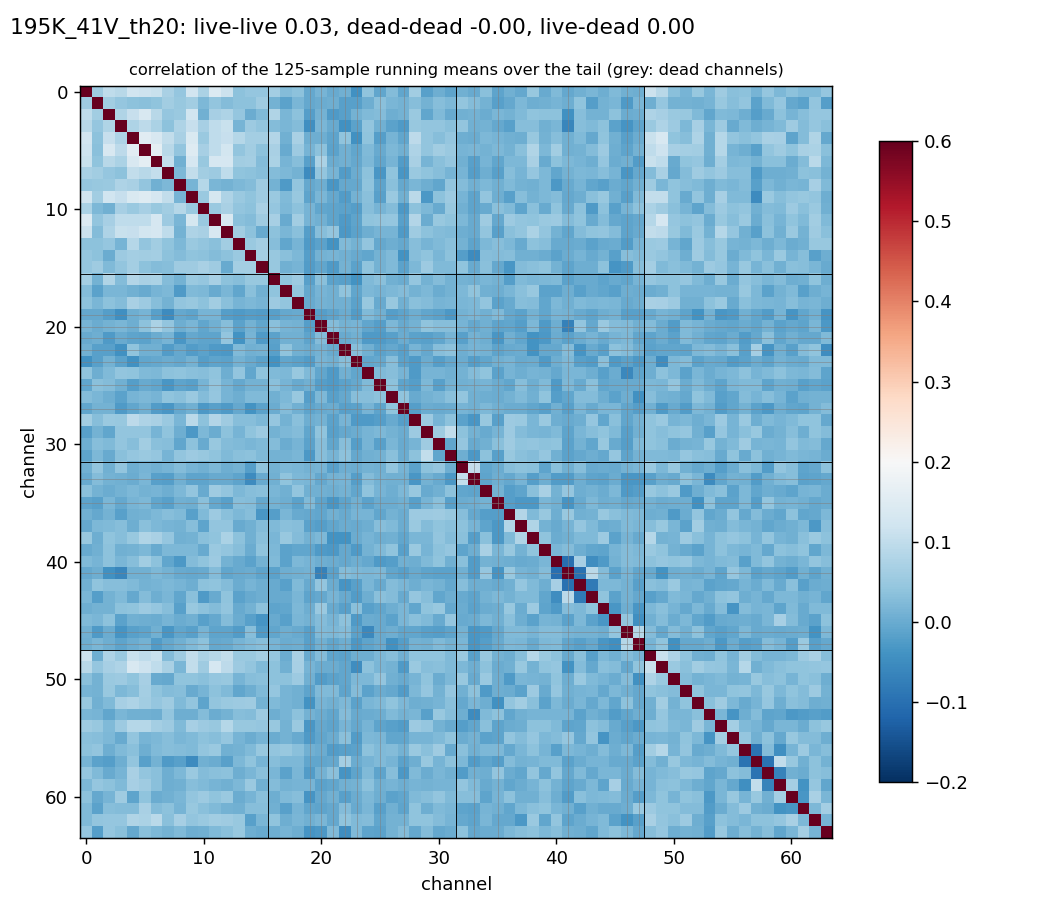
\includegraphics[width=0.75\linewidth]{cmnoise_195K_corr.png}
\caption{Correlation of the 125-sample running means over the tail,
channel against channel. Grey lines: dead channels. Black lines: the
digitizer groups of 16.}
\label{fig:corr}
\end{figure}

\begin{figure}[tbp]
\centering
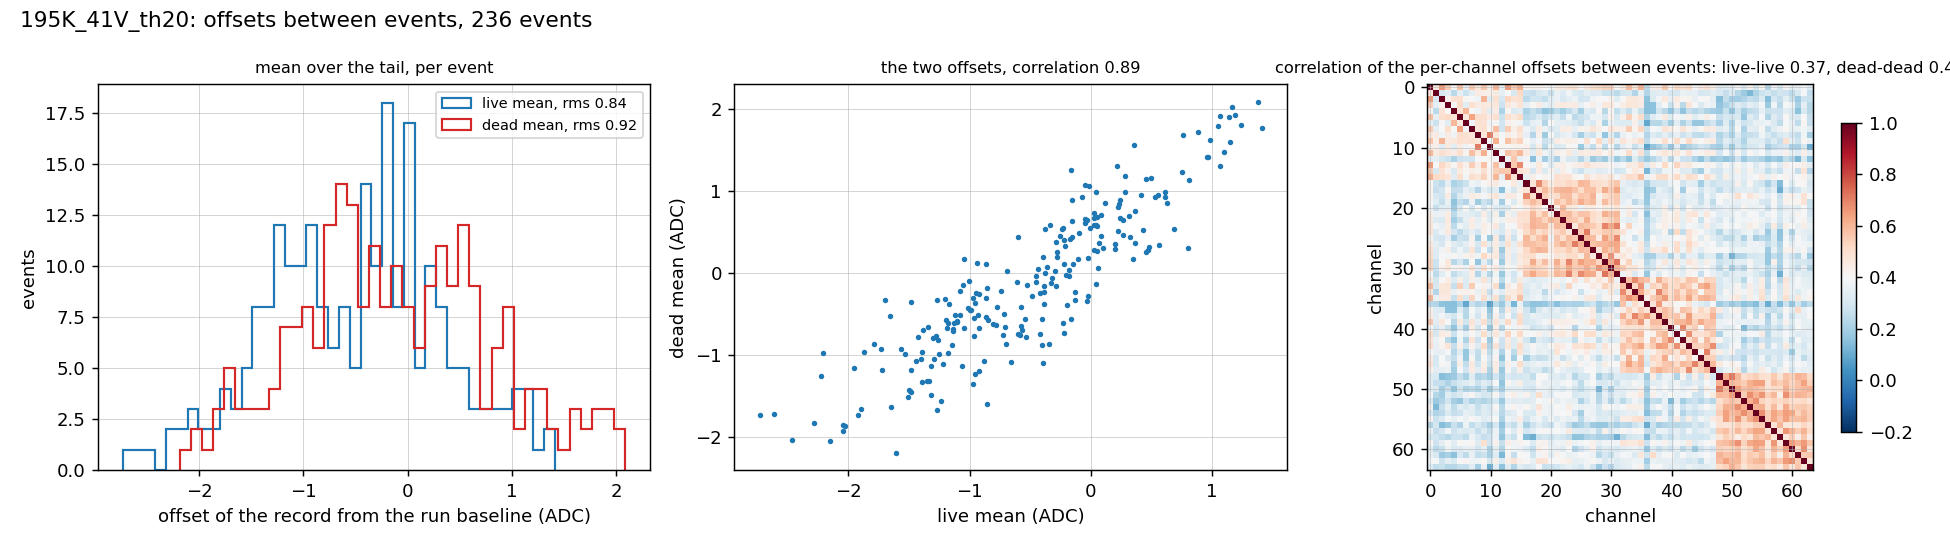
\includegraphics[width=\linewidth]{cmnoise_195K_offsets.png}
\caption{Offsets of the record from the run baseline between events: the
live and dead means, their correlation, and the correlation of the
per-channel offsets between events, with the blocks of the digitizer
groups.}
\label{fig:offsets}
\end{figure}

\subsection{Predicted noise in the signal window}

\paragraph{Method.} The charge of a window with no signal in it: the
5~\us geometry of the real window placed in the tail, its samples summed
minus a baseline, times 8~ns, over channels and events. Its rms is the
noise that baseline leaves on a real charge. Four baselines: the mean of
the last 250 samples of the record; the mean of the 2~\us right after
the window; a line fitted on the 1~\us before and the 6~\us after the
window; and, for the sum, the first of these after subtracting from
every channel the running mean of the twelve dead channels.

\paragraph{Prediction.} From the memory of 1.5~\us of the slow
component, the samples adjacent to the window carry information on its
first and last microsecond and none on its middle: the baseline from the
adjacent samples on both sides does best, the one from the far end of the
record worst, and the floor is the slow noise within the window itself.
From the independence of the channels, a baseline built from other
channels adds their noise: $n\,\sigma_{\rm ch}/\sqrt{n_{\rm ref}}$ on a
sum of $n$ channels from $n_{\rm ref}$ reference channels, 52\,000
ADC\,ns for 52 channels and the 12 dead ones, in quadrature with the
29\,000 of the raw sum: 59\,700.

\paragraph{Measurement.} Table~\ref{tab:empty} and
Figures~\ref{fig:examples} to~\ref{fig:sum}.

\begin{table}[h]
\centering
\begin{tabular}{l r r r}
\toprule
Baseline & dead channels & live channels & sum of 52 live \\
\midrule
white noise, 3.8 counts & 756 & 756 & 5\,400 \\
line on 1~\us before and 6~\us after & 2\,540 & 2\,670 & 26\,600 \\
mean of the 2~\us after & 3\,044 & 3\,130 & 26\,600 \\
mean of the last 250 samples & 3\,473 & 3\,581 & 29\,000 \\
the same after the dead-channel common mode & 3\,350 & 3\,719 & 60\,000 \\
\bottomrule
\end{tabular}
\caption{Rms of the charge of an empty 5~\us window, in ADC\,ns, over
236 events of \code{195K\_41V\_th20}.}
\label{tab:empty}
\end{table}

\begin{figure}[tbp]
\centering
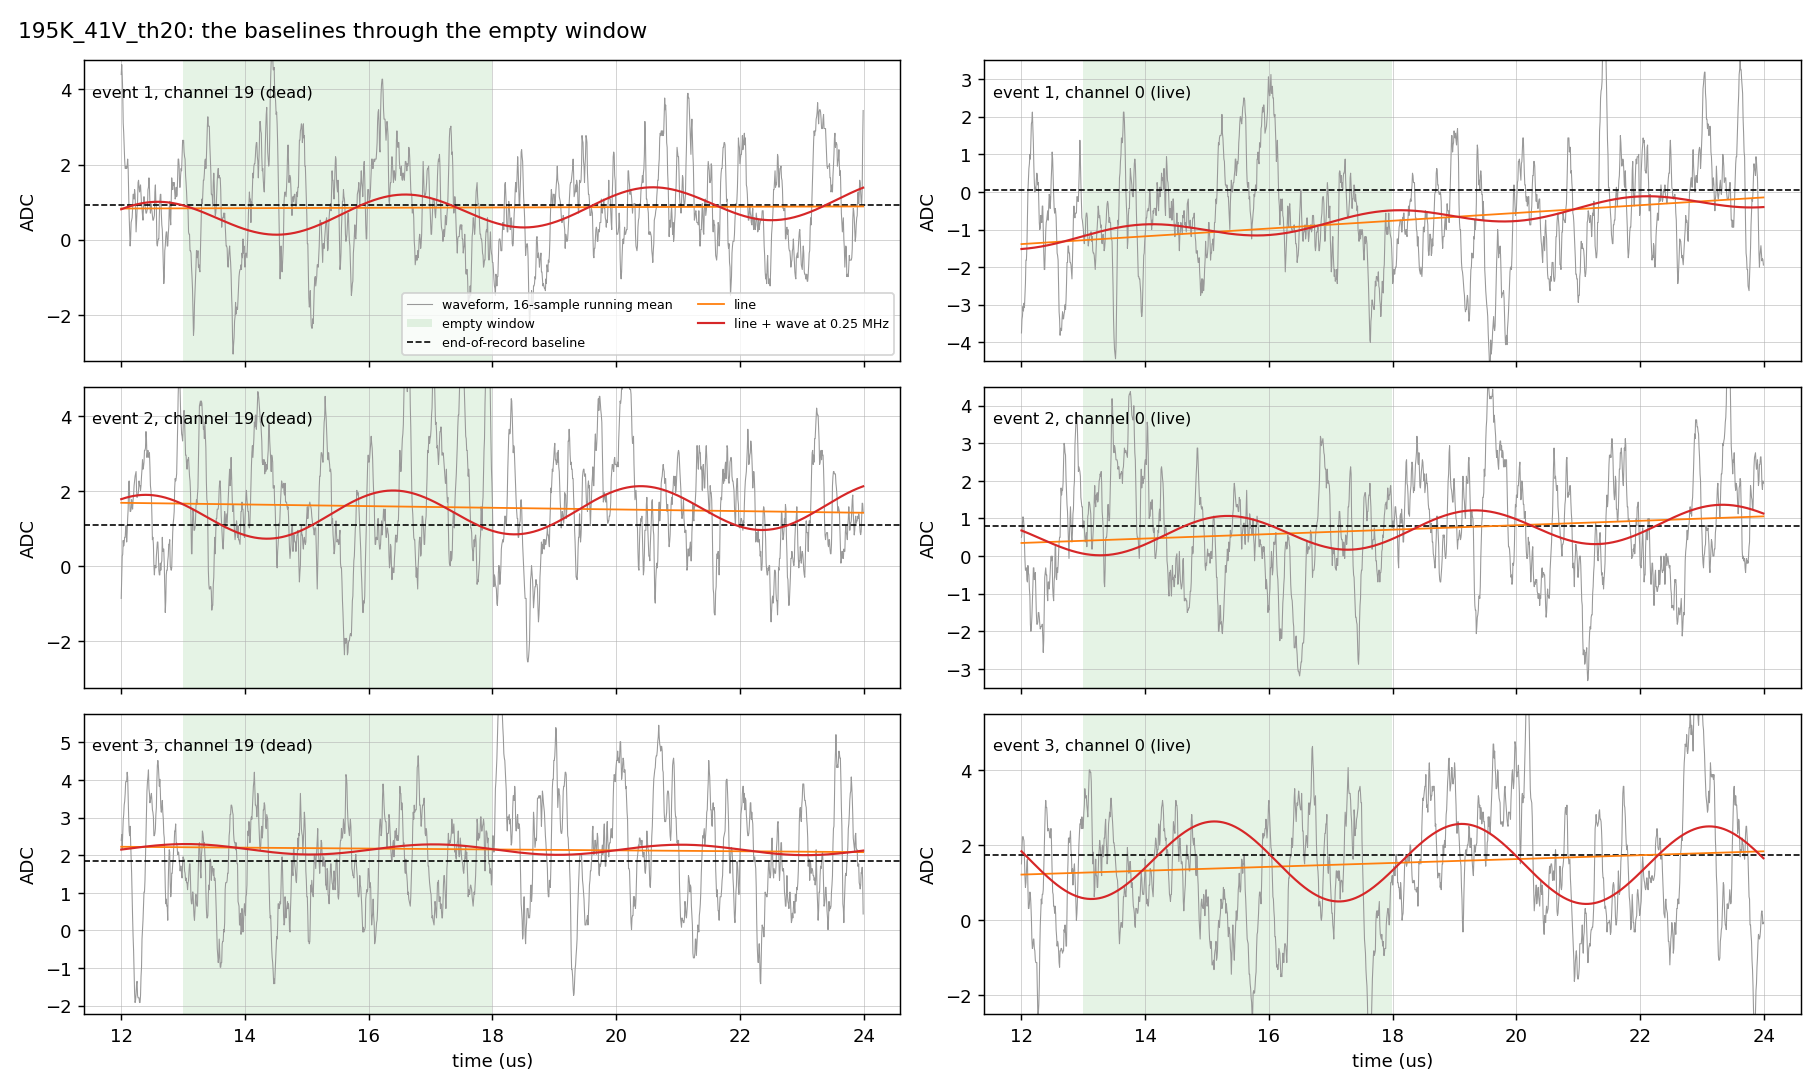
\includegraphics[width=\linewidth]{wavefit_195K_examples.png}
\caption{Three events, one dead and one live channel: the waveform over
the tail, the empty window, and the baselines through it.}
\label{fig:examples}
\end{figure}

\begin{figure}[tbp]
\centering
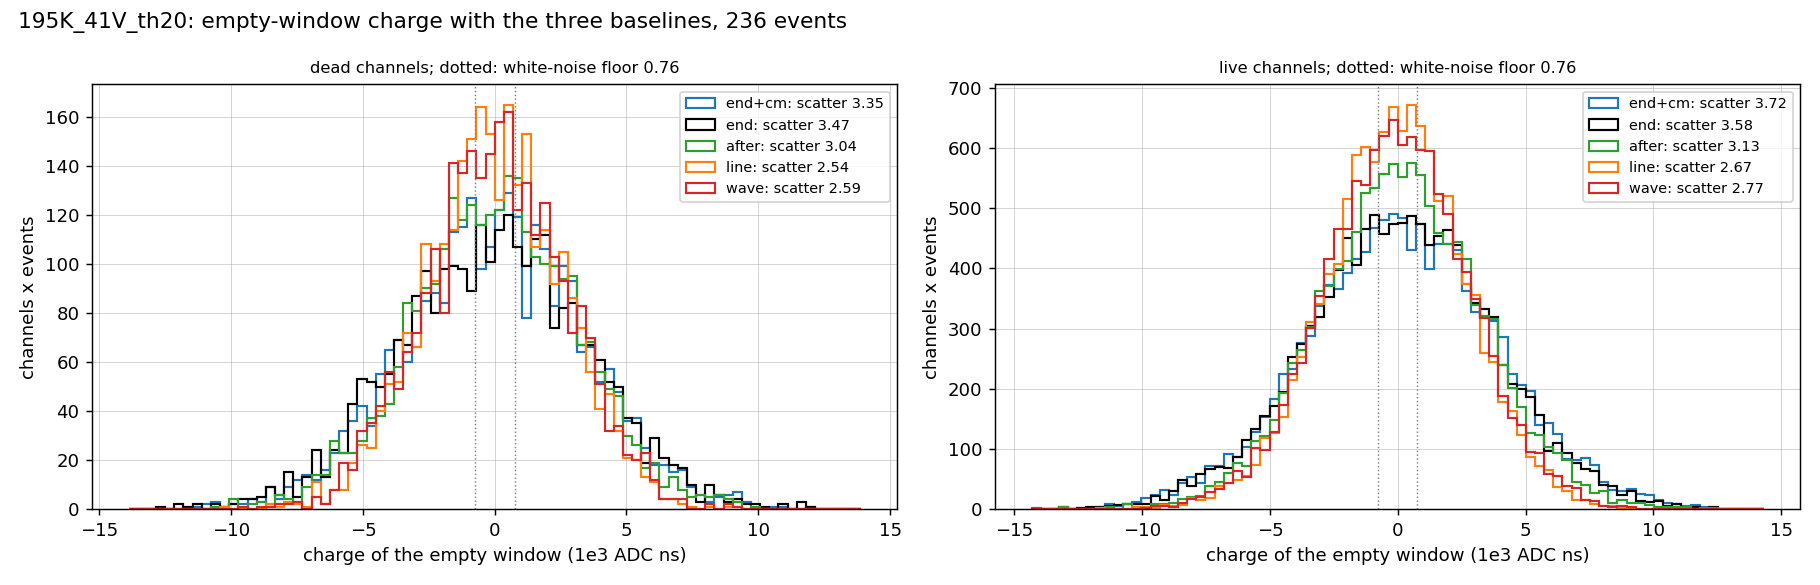
\includegraphics[width=\linewidth]{wavefit_195K_hist.png}
\caption{The charge of the empty window per baseline, dead and live
channels, with its rms; dotted, the white-noise floor.}
\label{fig:hist}
\end{figure}

\begin{figure}[tbp]
\centering
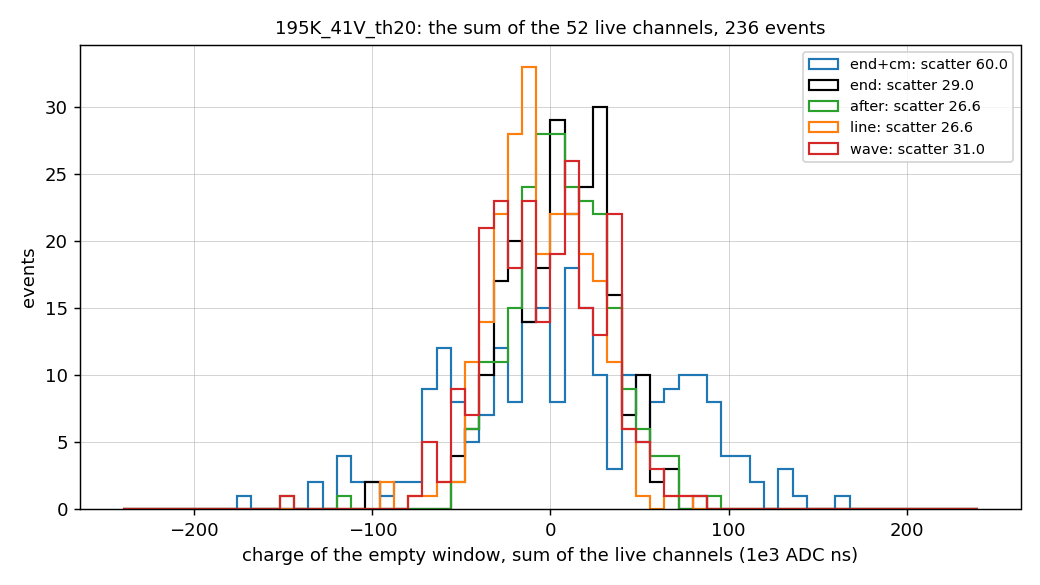
\includegraphics[width=0.7\linewidth]{wavefit_195K_sum.png}
\caption{The same for the sum of the 52 live channels, with the
dead-channel common mode as the fourth baseline.}
\label{fig:sum}
\end{figure}

\subsection{Noise correction}

Per channel, the baseline is the mean of the 1~\us before and the 2~\us
after the window. The window must have that room in the record, which
defines the SHORT class of Section~\ref{sec:selection}. No quantity is
subtracted across channels. A control charge per channel and event, the
same geometry on an empty stretch of the tail, measures the noise of
every estimator directly. The resulting noise is 2\,600 ADC\,ns per
channel and 27\,000 on the sum of 52. The residual, 3.4 times the white
floor, is the slow noise within the window, a property of the front-end;
a fit of the pulse shape inside the window is the one software handle
left on it, with a modest gain to expect.

\section{The single photoelectron}
\label{sec:spe}

The gain of a channel is the size of the pulse of one photoelectron. We
need it for three things: to put the 64 channels on the same scale before
summing them, to express the light yield in photoelectrons rather than in
counts, and, through its dependence on the bias, to measure the breakdown
voltage. There is no dedicated single-photoelectron run; the pulses have
to be found among the dark pulses in the part of the records that holds no
scintillation light, the last 10~\us.

\subsection{The pulse shape}

Figure~\ref{fig:template} shows the shape of the pulse, obtained from
13\,845 dark pulses of the run at 195~K and 41~V, where the pulses are
largest. The pulses were found as local maxima of the raw channel above 20
counts, a high threshold so that most of them are real, aligned on their
maximum sample, corrected for the local level by the median of the samples
before the peak, and averaged. The pulse rises in two samples, 16~ns, is
3.0 samples wide at half maximum, 24~ns, and decays over six samples,
50~ns. The same average from the first 300 events and from 2000 events
agrees to the third decimal. It carries a known defect: a pulse passes the
threshold more easily when the noise on its peak sample is positive, so
the central sample of the average is inflated, by about one count in
thirteen, and the shape is slightly too sharp. The normalised shape,
peak~1, is the template used below.

\begin{figure}[tbp]
\centering
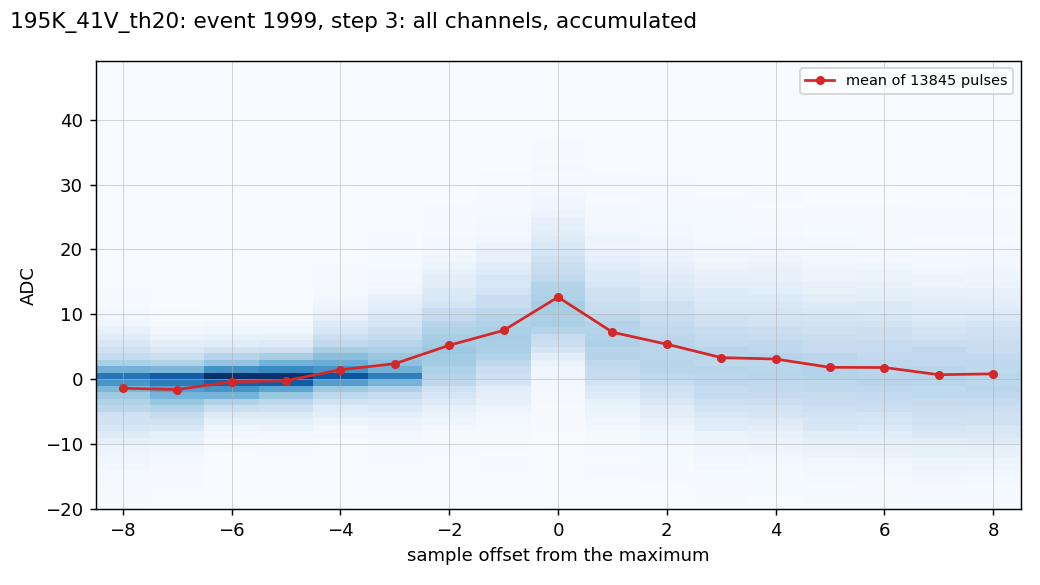
\includegraphics[width=0.75\linewidth]{figs/tpl_195K_s3.png}
\caption{The dark pulses of \code{195K\_41V\_th20} above 20 counts, aligned on
their maximum: the two-dimensional histogram of the amplitude against the
sample offset from the maximum, and the mean (points). The pre-peak samples
sit at zero after the local-level correction; the spread after the peak,
$\pm 10$ counts, is from pulses sitting on other pulses.}
\label{fig:template}
\end{figure}

\subsection{The spectra at 41 V and the equalization}

With the matched filter and a threshold at 4.5 times the filtered noise,
about 17 counts, the dark pulses of every channel of every event were
collected over the full run at 195~K and 41~V: 28\,664 candidates, 0.09
per channel and record, with the height of each one estimated by the
filter in counts of the raw peak. Figure~\ref{fig:spe} shows the spectrum
of the heights for one channel and for all live channels together, and
Figure~\ref{fig:spe_channels} the spectrum of every channel. In nearly
every live channel there is a peak at about 20 counts, cut on its low side
by the threshold, with a tail to the right from pulses with a crosstalk
partner and from overlapping pulses. The dead channels show only a spike
at the threshold, which is the contribution of noise maxima; it is a few
percent of the candidates of a live channel.

\begin{figure}[tbp]
\centering
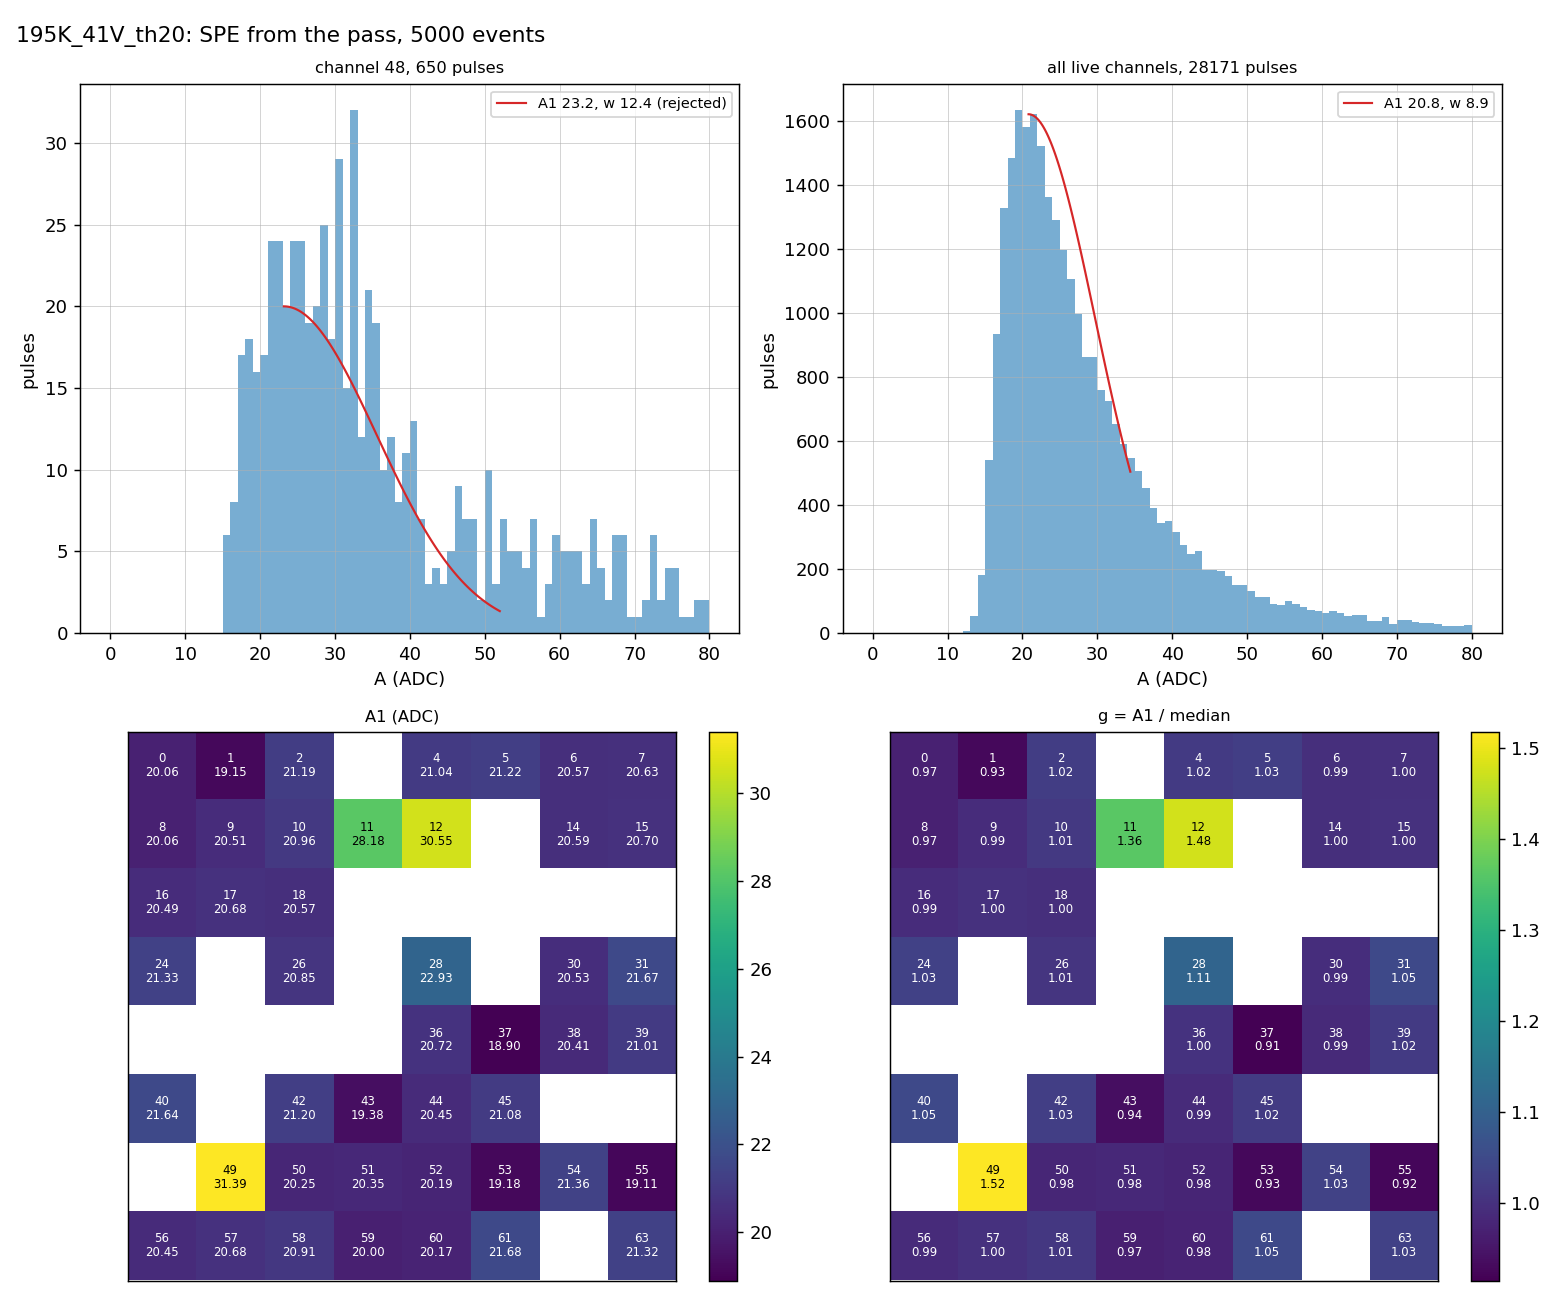
\includegraphics[width=\linewidth]{figs/spefit_195K.png}
\caption{Single-photoelectron spectra of \code{195K\_41V\_th20}, 5000 events.
Top left: channel 48. Top right: all live channels together, with the fit.
Bottom: the fitted amplitude $A_1$ per channel, and the equalization factor
$g_c = A_1 / 20.7$; empty cells are the dead channels and the channels
without an accepted fit.}
\label{fig:spe}
\end{figure}

\begin{figure}[tbp]
\centering
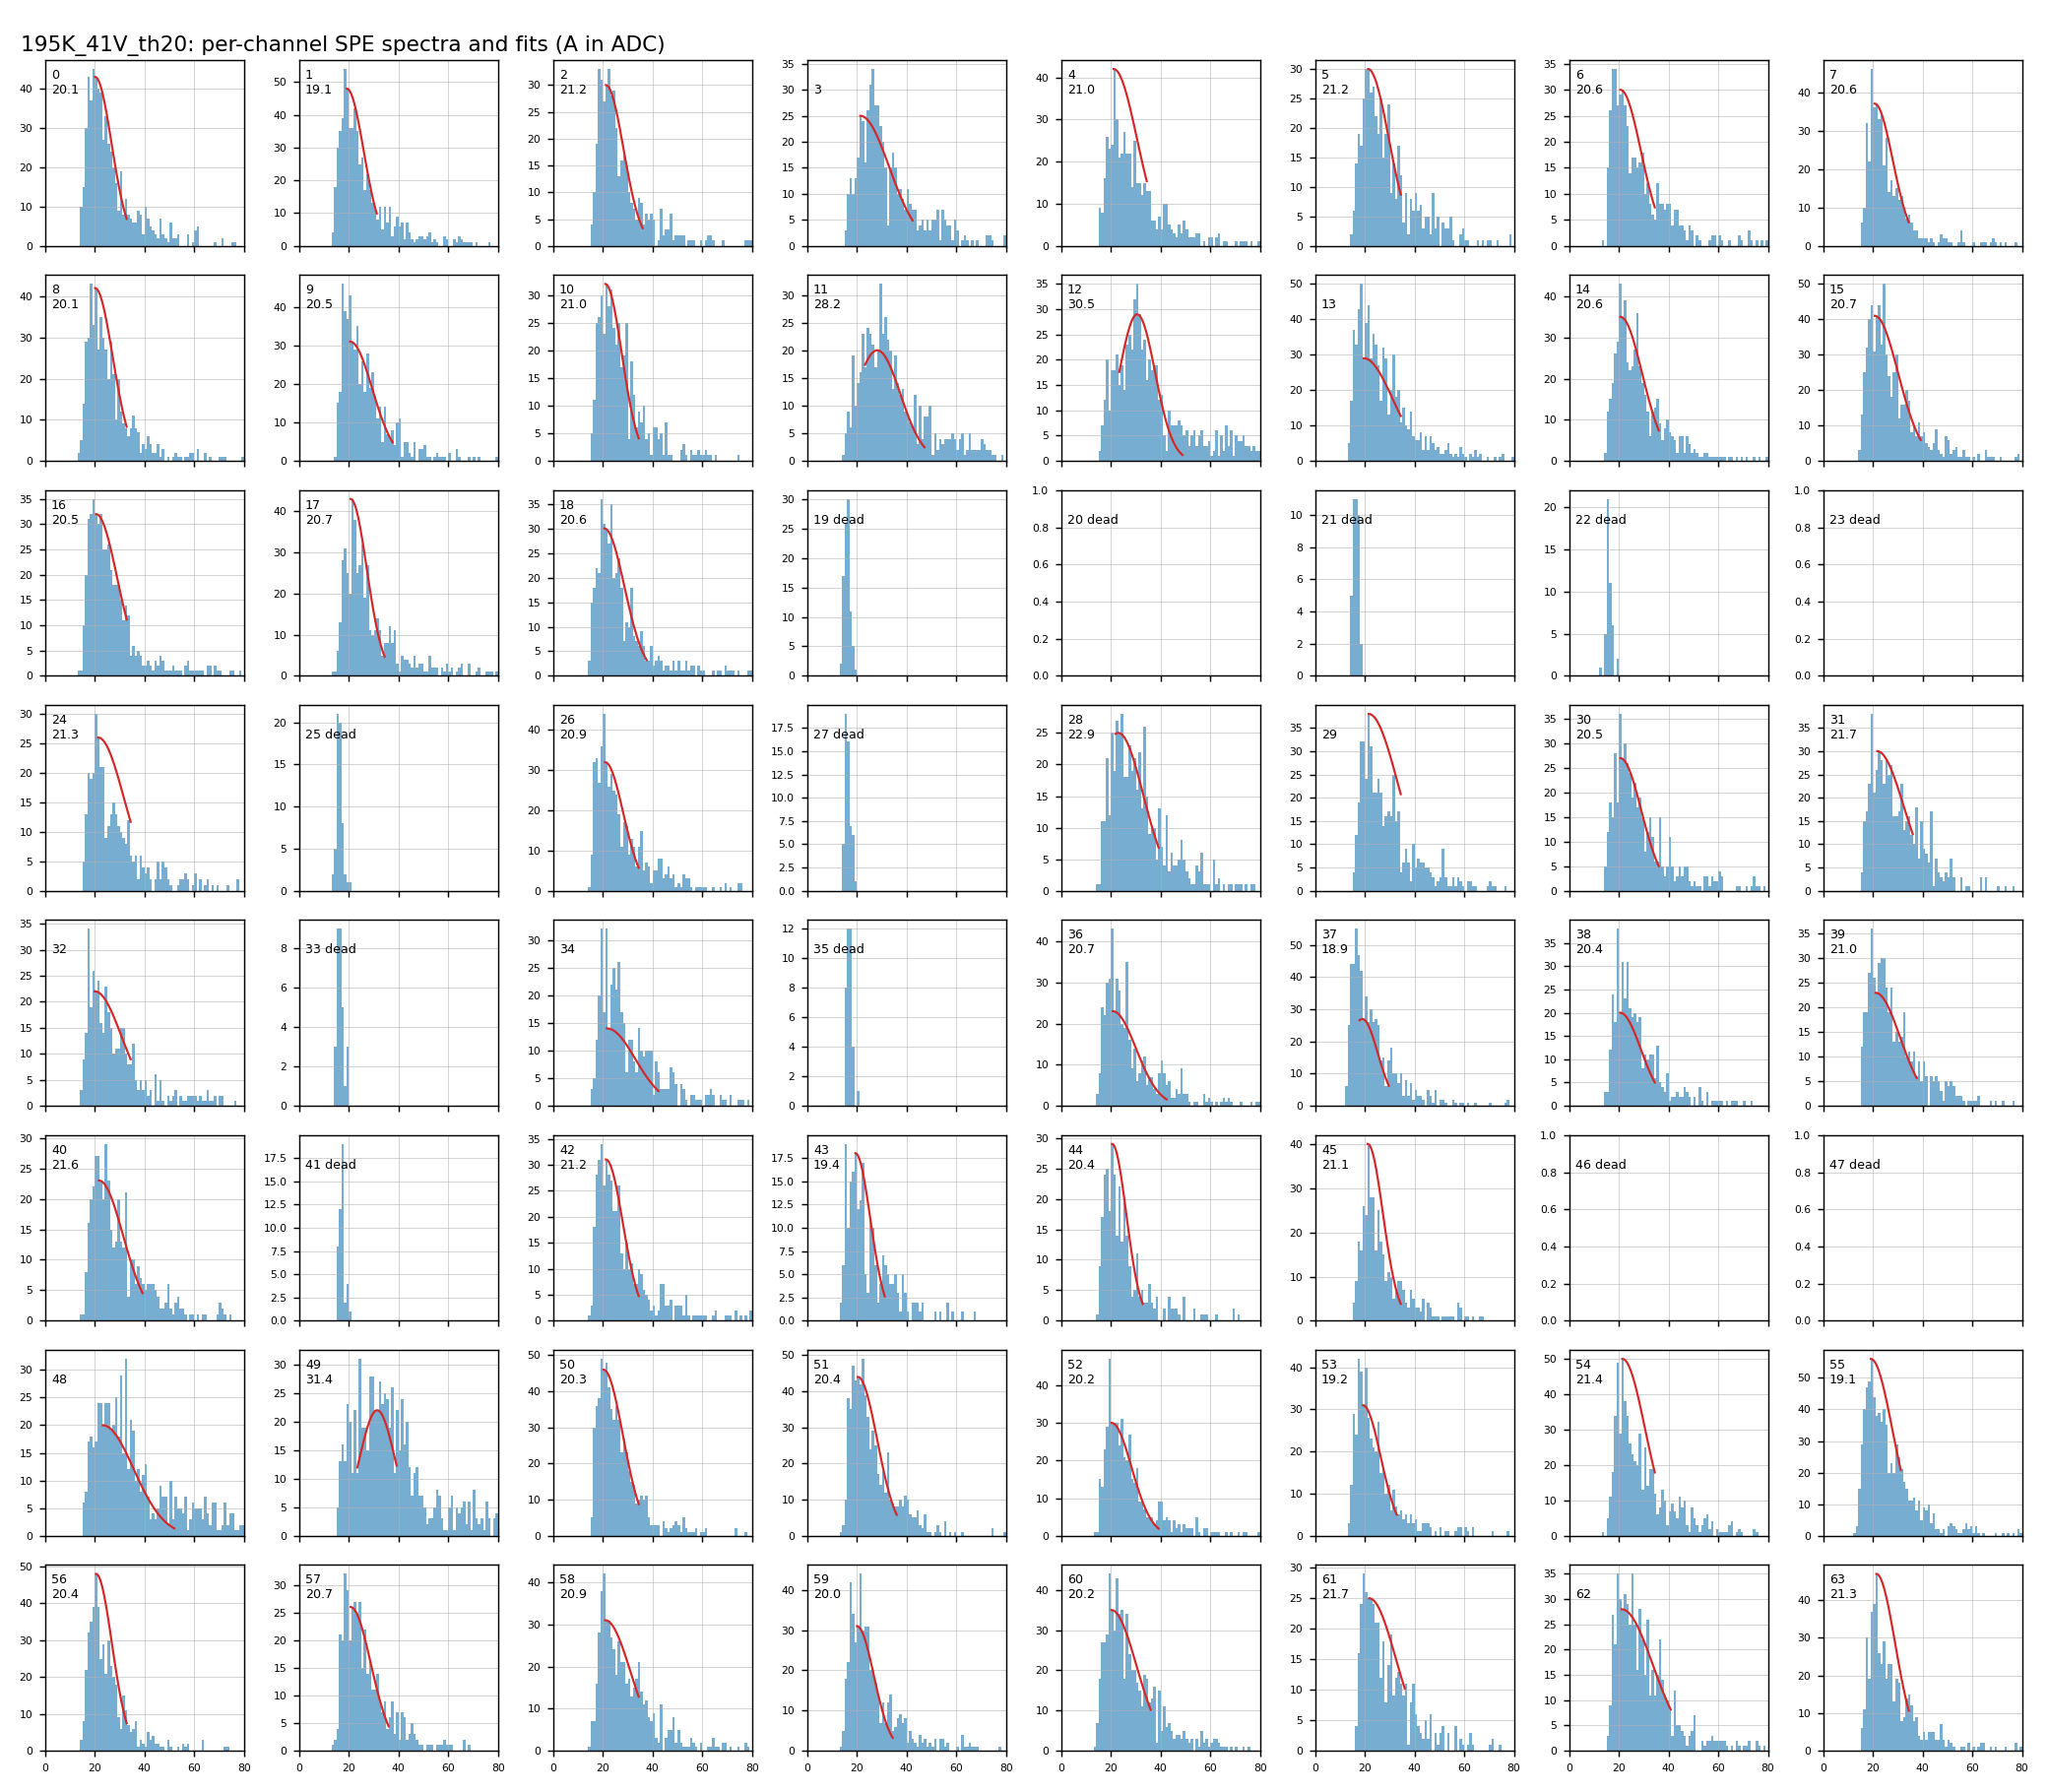
\includegraphics[width=\linewidth]{figs/spefit_195K_channels.png}
\caption{The spectrum of every channel, same run, with the fitted Gaussian
where the fit was accepted and $A_1$ in the corner. The dead channels show
only the spike at the threshold.}
\label{fig:spe_channels}
\end{figure}

The peak of each channel was fitted with a Gaussian from one noise width
above the threshold to 1.6 times the mode (fitting from the threshold
itself was tried; the Gaussian then stretches over the truncation and the
fit is worse). Forty-five of the 52 live channels give an accepted fit. The
median of the fitted amplitudes is 20.7 counts, and the normal channels
lie within $\pm 9\%$ of it, with errors of 1 to 4 counts each, which come
from the peak sitting only one noise width above the cut. The four
channels of Section~\ref{sec:channels} are where they were expected: 11 at
$28.2 \pm 1.5$ counts, 12 at $30.5 \pm 0.6$, 49 at $31.4 \pm 0.7$, that is
1.36, 1.48 and 1.52 times the median. Channel 48 has two populations, one
at the normal 22 counts and one at 33, and no single peak to fit; its gain
will have to come from its response to the scintillation light. The dark
rate of the live channels, from the number of candidates and the search
time, is 8 to 15~kHz at this overvoltage.

The equalization factor of a channel is $g_c = A_1(c) / 20.7$, and the
table of the 45 factors is in \code{src/spe\_gain\_195K\_41V\_th20.csv}.
Dividing each channel by its factor before summing puts the 64 channels in
the units of the median channel.

\subsection{The bias scan: breakdown voltage, and the nature of the four channels}

The same collection and fit were done on the other four runs of the bias
scan at 196~K, at 40.5, 40, 39.5 and 39~V. For the normal channels the
result is not a measurement: the number of candidates falls from 28\,664
at 41~V to 2705 at 39~V, while the fitted amplitude stays at 20 to 21
counts whatever the bias. The true peak slides down with the overvoltage,
from 20.7 counts to about 14 at 39~V, below the 17-count threshold, and
what the fit sees is the remnant above the cut, pinned just above it. The
normal channels can be followed only at 41~V.

The four high-gain channels can be followed further, because their peak
stays above the cut. Channel 49, the cleanest, gives $31.4 \pm 0.7$,
$29.2 \pm 1.5$ and $26.7 \pm 2.3$ counts at 41, 40.5 and 40~V: a slope of
4.7 counts per volt, which extrapolates to zero at 34.3~V. That is the
breakdown voltage of this SiPM at the temperature of the run. The datasheet
line gives 34.5~V at T3 and 34.9~V at T2, so the breakdown at 196~K is
where the extrapolation from the datasheet puts it, within half a volt,
and the data cannot tell whether the SiPMs were at the crystal temperature
or at that of the frame, as expected from the 0.3~V that separates the two
hypotheses.

The slope also says what the four channels are. If their larger gain came
from a lower breakdown voltage, their excess over the normal channels
would grow as the bias is lowered, since the ratio $(V - V_{\rm bd}^{\rm
ringer}) / (V - V_{\rm bd}^{\rm normal})$ grows as $V$ approaches the normal
breakdown. Dividing the amplitude of channel 49 by the normal amplitude
scaled with the overvoltage, $20.7\,(V - 34.5) / 6.5$, gives 1.52, 1.53,
1.53 and 1.48 at 41, 40.5, 40 and 39.5~V: constant. A constant factor is a
larger gain after the SiPM, in the shaper of that channel. The same holds
for 11 and 12 within their larger errors. The practical consequence is
welcome: the equalization factors do not depend on the bias or the
temperature, and the table from the 41~V run applies to every run,
including the cold ones where no dark pulse can be seen.

What this leaves open is stated plainly. The single-photoelectron
amplitude of the normal channels is measured at one point, 41~V and 196~K,
and the gain of every other run has to come from the datasheet dependence
of the gain on the overvoltage, anchored at that point and checked by the
light itself: the position of the 511~keV photopeak along the bias scans
is the next measurement of the same quantity, and it is where the analysis
note begins.

\section{Event selection}
\label{sec:selection}

One pass per run, in Julia (\code{src/jscan}), one output file per run.
Nothing is subtracted across channels.

\subsection{The windows of the run}

From the average pulse of the run, before any pass: the charge window
starts 1~\us before the maximum and ends a fixed multiple of the decay
time after it, so that every temperature integrates the same fraction of
the light. The pass reads the window from a per-run table; the record
length and the pre-trigger come from the file.

\paragraph{Figure.} The average pulse of the run, linear and
logarithmic, the window shaded, the decay fit drawn.

\subsection{The pulse search}

On the sum of the live channels, each divided by its gain factor: the
running mean over 64 samples, its maximum and time $t_{\max}$, the
height $H$ against the rms of the smoothed sum in a pulse-free region,
the rising edge as the last sample below $H/2$ before the maximum.

\paragraph{Figure.} Per run, the distribution of $H$ over the smoothed
noise, with the cut, and the distribution of $t_{\max}$, with the
pre-trigger and the SHORT boundary marked.

\subsection{The classes}

Decided in this order on every event: EMPTY, no pulse above the cut;
TAIL, a pulse without rising edge, started before the record; SHORT, a
rising edge but less than 1~\us of record before the window or 2~\us
after it; REAL otherwise, with a pile-up flag when a second maximum
stands beyond the window and its veto, separated by a valley.

\paragraph{Figure.} The height spectrum by class and the fractions per
run; across runs, the SHORT fraction against the board trigger rate,
which measures how late the trigger fires at each bias.

\subsection{The single-photoelectron candidates}

In the last 10~\us of every event of every class, with the matched
filter of Section~\ref{sec:spe}, skipping the events whose second
maximum falls inside the search region. SHORT events contribute as
much as REAL ones: the search does not depend on the window.

\paragraph{Figure.} The number of candidates per class; the amplitude
spectrum with its fit for one channel and the map of the gains.

\subsection{The charge per channel}

For REAL events only. Per channel, the baseline is the mean of the 1~\us
before and the 2~\us after the window, both always available by
construction of the class; the charge is the sum of the samples over
the window minus the baseline, times 8~ns; the time of the channel
maximum is kept; and a control charge is taken with the same geometry on
an empty stretch of the tail, the noise reference of that event and
channel.

\paragraph{Figure.} One event, one channel: the waveform, the window,
the two baseline stretches and the level. Per run, the width of the
control charge per channel on the map.

\subsection{The output}

Per event: index, trigger id, timestamp, $t_{\max}$, window, $H$, class,
flags, time of the second maximum; for REAL events the 64 charges, the
64 control charges and the 64 channel times; the summed waveform for the
average pulse; as metadata the run conditions, the parameters and the
commit.

\section{Event analysis}
\label{sec:analysis}

Per run, in Python (\code{offline.py}), from the pass file.

\subsection{The sample}

REAL events without pile-up. The fraction removed as SHORT is reported
per run. The trigger fires earlier on brighter pulses, so the selection
could favour them: the check is the photopeak position against the SHORT
fraction across the runs of a bias scan.

\paragraph{Figure.} Photopeak position against SHORT fraction, one point
per run.

\subsection{Equalization}
\label{sec:equalization}

The gain table of Section~\ref{sec:spe}; channel 48 and the seven
channels without an accepted fit, from their light response in the
photopeak events.

\paragraph{Figure.} The gain map and the light-response map, before and
after equalization.

\subsection{The response correction}
\label{sec:response}

The response depends on where the light lands. Grouping the events by
seed channel, the channel with the largest equalized charge, the
photopeak position differs from channel to channel by 11\% rms, from 0.76
to 1.21 of the median, lowest in the ring of channels around the dead
block and highest far from it; the spread is the same on the unequalized
charge, so it is light collection and not gain. Uncorrected, an 11\% rms
spread of the response broadens the photopeak by 26\% FWHM. First
correction: per seed channel, dividing the event's charge by the photopeak
position of its group; it brings the 511~keV width from 46 to 22\% at
41~V. Then per channel from the data, the 52 factors that bring the
photopeak events to one value, applied to the charges before the sum.

\paragraph{Figure.} The map of the per-seed-channel peaks before and
after, and the photopeak before and after.

\subsection{The estimators}

The equalized sum of all live channels is the reference; the sum of the
positive charges and the zero-suppressed sum are kept for comparison.
The same sums over the control charges give the noise of each estimator
directly, event by event.

\paragraph{Figure.} The spectra of the estimators with their fits and,
beside each, the spectrum of its control charge with its width.

\subsection{The photopeaks}

The 511~keV line and the 1275~keV line, each a Gaussian on a Compton
step. Light output as the position in ADC\,ns and in photoelectrons;
resolution as FWHM over position. The ratio of the two positions is the
linearity and the trigger check.

\paragraph{Figure.} The spectrum with both fits and the step.

\subsection{The decay time}
\label{sec:decay}

From the average pulse of the REAL events, one or two exponentials over
a range set per run. At 196~K the average pulse is a single exponential
of $2.74 \pm 0.01$~\us.

\paragraph{Figure.} The average pulse with the fit, linear and
logarithmic.

\section{Energy resolution}
\label{sec:resolution}

Per run, the width of the 511~keV peak and its budget, each term measured
and compared in quadrature with the width:
\begin{itemize}
\item the electronic noise, from the control charge of the estimator;
\item the photoelectron statistics, from the position in photoelectrons,
  with the excess from crosstalk and afterpulsing estimated from the
  charge of a single photoelectron against its amplitude;
\item the response non-uniformity, from the spread of the per-channel
  peaks before and after the correction;
\item the equalization error, bounded by the errors of the gain table;
\item the Compton continuum under the peak, from the step of the fit;
\item the remainder: the crystal, and what has not been found.
\end{itemize}

\paragraph{Figure.} The terms stacked in quadrature per run against the
measured width.

\section{Results}

\subsection{Light output}

The 511~keV position in ADC\,ns and in photoelectrons at the two
overvoltages, raw and corrected for the overvoltage: gain linear in
overvoltage, breakdown voltage from Section~\ref{sec:spe}, photon
detection efficiency taken as saturated; the crosstalk and afterpulsing
excess against overvoltage stated as the main systematic.

\subsection{Decay time}

The two values with their errors.

\subsection{Energy resolution}

The width at the two overvoltages with its budget, from
Section~\ref{sec:resolution}, in one line each.

\subsection{Summary table}

One line per run: T3, bias, overvoltage, trigger rate, class fractions,
light output, decay time, resolution, 511 to 1275 ratio.

\end{document}
